% ------------------------------------------------------------------------
%
% -------------------      Plantilla_UIS.tex       -----------------------
%
% ------------------------------------------------------------------------
% ------------------------------------------------------------------------
% ------------------------------------------------------------------------
% Versi�n de plantilla para realizaci�n de informes de trabajo de grado
% construida para uso de la Universidad Industrial de Santander.
%
% Reservados todos los derechos
%
% Bucaramanga, Colombia
%
% Febrero 03 de 2019
%
% ------------------------------------------------------------------------
% ------------------------------------------------------------------------
% ------------------------------------------------------------------------
%
% ------------------------------------------------------------------------
\documentclass[letter,oneside,12pt,spanish]{report}          % Encabezados
% ------------------------------------------------------------------------
\usepackage{uislatexstyleAPA}                           % Libreria UIS APA
% ------------------------------------------------------------------------
% Ingrese en este punto las librer�as espec�ficas de usuario
% ------------------------------------------------------------------------
\usepackage{epsfig}
\usepackage{amsmath}
\usepackage{amssymb}
\usepackage{subfigure}
\usepackage{longtable}
\usepackage{lscape}
\usepackage{float}
\usepackage{listings}
\usepackage{xcolor}
\usepackage{textcomp}
\lstset{
	basicstyle=\ttfamily,
	columns=fullflexible,
	frame=single,
	breaklines=true,
	postbreak=\mbox{\textcolor{red}{$\hookrightarrow$}\space},
}

% ------------------------------------------------------------------------
\begin{document}                                     % Inicio de documento
% ------------------------------------------------------------------------
% Definici�n sil�bica de palabras
% ------------------------------------------------------------------------
\hyphenation{pro-por-cio-nal di-se-�o}
% ------------------------------------------------------------------------
% Titulo resumido del trabajo que aparecer� en cornisa
% ------------------------------------------------------------------------
\title{Definici�n de una infraestructura cloud}
% ------------------------------------------------------------------------
% Elementos previos al contenido del trabajo
% ------------------------------------------------------------------------
% ------------------------------------------------------------------------
%                               Portadilla
% ------------------------------------------------------------------------

\begin{center}

Definici�n de una infraestructura cloud de alta disponibilidad en un entorno distribuido para el despliegue de una plataforma IoT	 \vspace{2.3cm}

Jose David Rojas Aguilar\\ \vspace{2.3cm}

Trabajo de Grado para optar al t�tulo de Ingeniero de Sistemas\\ \vspace{2.3cm}

Director\\
Gabriel Rodrigo Pedraza Ferreira\\
Doctor en Ciencias de la computaci�n \vspace{2.4cm}

Universidad Industrial de Santander\\
Facultad de Ingenier�as Fisicomec�nicas\\
Escuela de Ingenier�a de sistemas e inform�tica\\
Bucaramanga\\
2019\\


\end{center}

% ------------------------------------------------------------------------
%                             Nota de proyecto
% ------------------------------------------------------------------------

\newpage

\begin{figure}
\begin{center}
\includegraphics[width=1.0\textwidth]{figs/nota}
\end{center}
\end{figure}

% ------------------------------------------------------------------------
%                             Autorizaci�n
% ------------------------------------------------------------------------

\newpage

\begin{figure}
\begin{center}
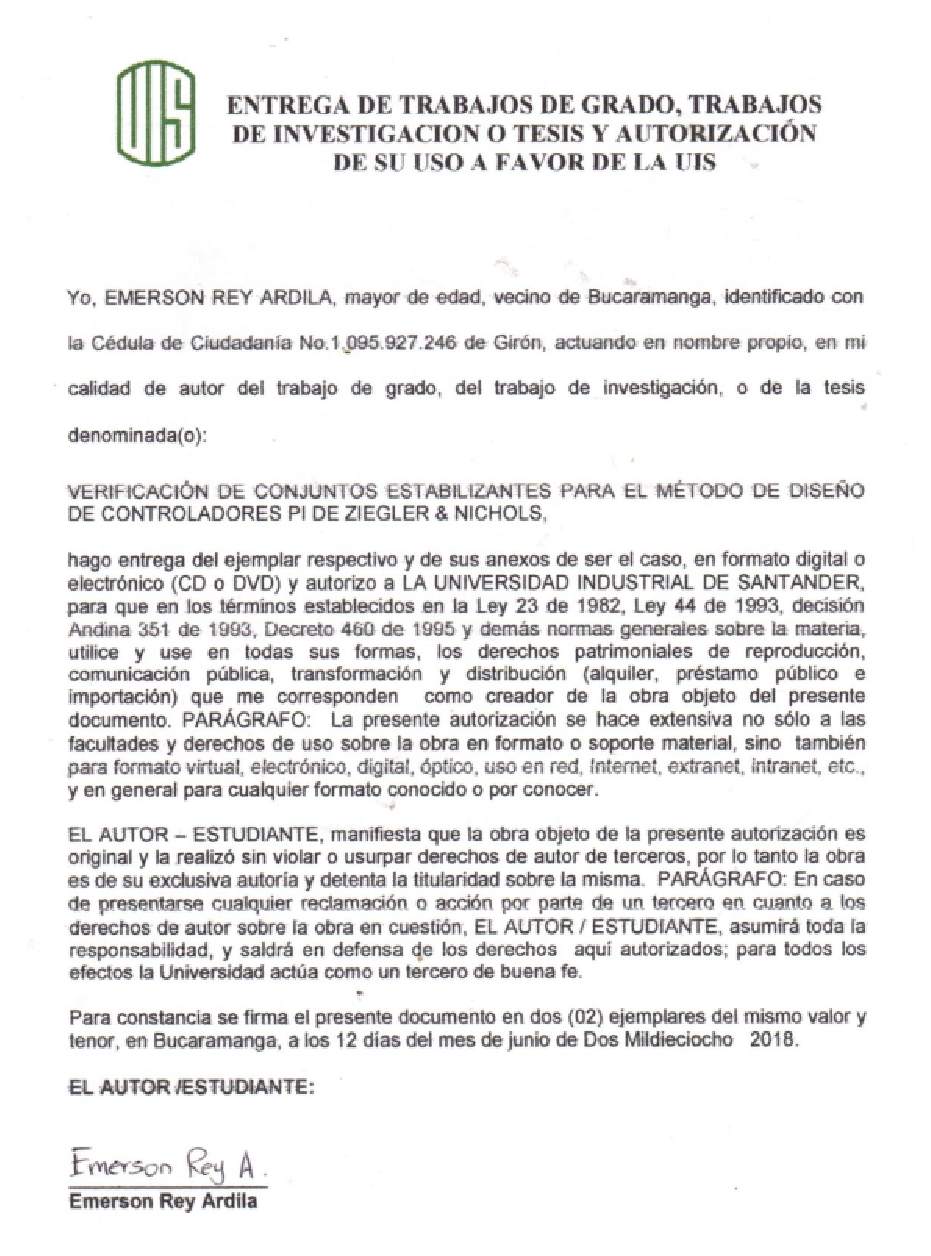
\includegraphics[width=0.9\textwidth]{figs/autoriza}
\end{center}
\end{figure}
% ------------------------------------------------------------------------              % Portadilla, formato de nota y autorizaci�n
% ------------------------------------------------------------------------
% ------------------------------------------------------------------------
% ------------------------------------------------------------------------
% ------------------------------------------------------------------------
%                               Dedicatoria
% ------------------------------------------------------------------------
% ------------------------------------------------------------------------
% ------------------------------------------------------------------------
\chapter*{Dedicatoria}

\noindent Este trabajo viene dedicado para todas aquellas personas que apoyaron el desarrollo
y ejecuci�n de este trabajo de grado.\\

En especial reconozco la permanente presencia de Dios en mi camino de vida.
% ------------------------------------------------------------------------                                    % Dedicatoria
% ------------------------------------------------------------------------
% ------------------------------------------------------------------------
% ------------------------------------------------------------------------
% ------------------------------------------------------------------------
%                             AGRADECIMIENTOS
% ------------------------------------------------------------------------
% ------------------------------------------------------------------------
% ------------------------------------------------------------------------
\chapter*{Agradecimientos}

%\noindent 
% ------------------------------------------------------------------------
\newpage                            % Agradecimientos
% ------------------------------------------------------------------------
\tableofcontents                                      % Tabla de contenido
% ------------------------------------------------------------------------
\listoffigures                         % Lista de figuras, tablas y anexos
\listoftables
\listofanexo
% ------------------------------------------------------------------------
% ------------------------------------------------------------------------
% ------------------------------------------------------------------------
% ------------------------------------------------------------------------
%                                Glosario
% ------------------------------------------------------------------------
% ------------------------------------------------------------------------
% ------------------------------------------------------------------------
\chapter*{Glosario}

\begin{description}
  \item[Backend] Capa  software  que  se  encarga  de  gestionar  los  datos  de  una  o  varias aplicaciones.
  \item[Continuous deployment] Pr�ctica que consiste en realizar el proceso de despliegue de forma autom�tica al ambiente de producci�n.
  \item[Dataset] Conjunto de datos generados o extra�dos de una fuente para su posterior procesamiento.
  \item[Development \& Operations] Es una pr�ctica de ingenier�a de software que tiene como objetivo automatizar y monitorear las etapas del ciclo de vida del software..
  \item[Infraestructura] Conjunto de componentes inform�ticos que permiten mantener un conjunto de aplicaciones al servicio de usuarios.
  \item[Internet de las cosas] Es un sistema de dispositivos de computaci�n interrelacionados con la capacidad de transferir datos a trav�s de una red, sin requerir intervenci�n humana.
  \item[Sistema de alimentaci�n ininterrumpida] Dispositivo que almacena energ�a para suministrar a equipos en caso de alguna falla el�ctrica
\end{description}
% ------------------------------------------------------------------------                              % Glosario de t�rminos
% ------------------------------------------------------------------------
% Contenido del Informe
% ------------------------------------------------------------------------
% ------------------------------------------------------------------------
% ------------------------------------------------------------------------
% ------------------------------------------------------------------------
%                                Resumen
% ------------------------------------------------------------------------
% ------------------------------------------------------------------------
% ------------------------------------------------------------------------
\chapter*{Resumen}

\footnotesize{
\begin{description}
  \item[T�tulo:] Definici�n de una infraestructura cloud de alta disponibilidad en un entorno distribuido para el despliegue de una plataforma IoT\astfootnote{Trabajo de grado}
  \item[Autor:] Jose David Rojas Aguilar \asttfootnote{Facultad de Ingenier�as F�sico-Mec�nicas. Escuela de Ingenier�a de sistemas e inform�tica. Director: Gabriel Rodrigo Pedraza Ferreria, Doctorado en Ciencias de la Computaci�n.}
  \item[Palabras Clave:] Infraestructura, Cloud, Alta disponibilidad, Definici�n, Cluster.
  \item[Descripci�n:] El internet de las cosas (IoT) ha tenido un gran impacto en los �ltimos a�os dentro de la sociedad en diferentes contextos. Una de sus aplicaciones mas importantes es la mejora de la calidad de vida y el apoyo en el proceso de aprendizaje de los estudiantes dentro de las diferentes universidades. Un reto dentro del IoT es tener una infraestructura capaz de soportar una cantidad masiva de dispositivos enviando informaci�n de forma constante. \\
  
  Este trabajo de investigaci�n se busca dise�ar una arquitectura software para el despliegue de una plataforma IoT en una infraestructura cloud de alta disponibilidad en un entorno distribuido. El proyecto inici� con una fase de exploraci�n con el fin de identificar las herramientas disponibles en el mercado. Luego se definieron unos criterios de selecci�n a nivel t�cnico, unos requisitos de los artefactos a desplegar, un conjunto de m�tricas y un conjunto de pruebas para evaluar el desempe�o de la arquitectura plateada. Despu�s se defini� una arquitectura la cual fue evaluada, en una primera oportunidad, por las pruebas dise�adas durante el proyecto y, finalmente, en una prueba de integraci�n en un caso de uso de la plataforma IoT.
\end{description}}\normalsize
% ------------------------------------------------------------------------                                                % Resumen
% ------------------------------------------------------------------------
% ------------------------------------------------------------------------
% ------------------------------------------------------------------------
%                                Abstract
% ------------------------------------------------------------------------
% ------------------------------------------------------------------------
% ------------------------------------------------------------------------
\chapter*{Abstract}

\footnotesize{
\begin{description}
  \item[Title:] Definition of a cloud infrastructure of high availability in a distributed environment for the deployment of an iot platform\astfootnote{Bachelor Thesis}
  \item[Author:] Jose David Rojas Aguilar\asttfootnote{Faculty of Physical-Mechanical Engineering. School of Systems Engineering and Informatics. Advisor: Gabriel Rodrigo Pedraza Ferreira, PhD in Computer science}
  \item[Keywords:] Infrastructure, Cloud, High availability, Definition, Cluster.
  \item[Description:] The Internet of Things (IoT) has had a strong impact in recent years within society in different contexts. One of its most important applications is the improvement of the quality of life and the support in the learning process of the students in different universities. A challenge in the IoT is to have an infrastructure capable of supporting a massive amount of devices sending information constantly. \\
  
  This research work looks for design software architecture for the deployment of an IoT platform in a high availability cloud infrastructure in a distributed environment. The project began with an exploration phase in order to identify the tools available in the market. Then technical selection criteria were defined, requirements of the artifacts to be deployed, a set of metrics and a set of tests to evaluate the performance of the proposed architecture. An architecture was defined, which was evaluated, at a first opportunity, by the tests designed during the project and, finally, in an integration test in a case of use of the IoT platform.
\end{description}}\normalsize
% ------------------------------------------------------------------------                                               % Abstract
% ------------------------------------------------------------------------
% Cap�tulos
% ------------------------------------------------------------------------
% ------------------------------------------------------------------------
% ------------------------------------------------------------------------
% ------------------------------------------------------------------------
%                              Introducci�n
% ------------------------------------------------------------------------
% ------------------------------------------------------------------------
% ------------------------------------------------------------------------

\nnchapter{Introducci�n}
% ------------------------------------------------------------------------
% ------------------------------------------------------------------------


\noindent La expansi�n de internet y los grandes avances la comunicaci�n entre diferentes dispositivos ha permitido el surgimiento de un nuevo paradigma tecnol�gico: Internet de las cosas (IoT). IoT se define como la infraestructura mundial para la sociedad de la informaci�n, que permite poner diferentes servicios a dispositivos interconectados entre s�, gracias a las tecnolog�as de la informaci�n y comunicaci�n, permitiendo la extracci�n y procesamiento masivo de datos. \\

El internet de las cosas ha tenido un impacto significativo en contextos de diferentes magnitudes. Grandes empresas como Amazon, Microsoft, Google, Cisco, Philips e Intel han invertido millones en investigaci�n, generando diferentes servicios enfocados al hogar, empresas e incluso ciudades. Barcelona es una ciudad pionera en el uso de IoT en sus calles, por ejemplo, la l�nea 9 del metro de Barcelona se ha actualizado con ascensores inteligentes que utilizan los datos en tiempo real para adaptarse a las necesidades de los viajeros lo cual ha logrado disminuir las aglomeraciones y el consumo de energ�a para 30 millones de pasajeros al a�o\citep{BARCELONA2019}. \\

Uno de los campos de aplicaci�n del IoT se encuentra en las universidades con el fin de mejorar la calidad de vida y apoyar el proceso de formaci�n en los estudiantes. La implementaci�n de una soluci�n IoT suele ser una tarea muy compleja que requiere de una infraestructura hardware y software capaz de soportar una cantidad masiva de dispositivos enviando informaci�n de forma continua por lo cual una caracter�stica fundamental dentro de una infraestructura IoT es la alta disponibilidad. \\

En este trabajo de investigaci�n se presenta el dise�o de una infraestructura para el despliegue de una plataforma IoT en una infraestructura cloud de alta disponibilidad en un entorno distribuido con el fin de proveer un entorno que pueda soportar una gran de dispositivos conectados enviado datos de forma masiva. 
   	% Introducci�n
% ------------------------------------------------------------------------
% ------------------------------------------------------------------------
% ------------------------------------------------------------------------
%                              Objetivos
% ------------------------------------------------------------------------
% ------------------------------------------------------------------------
% ------------------------------------------------------------------------

\chapter{Objetivos}
% ------------------------------------------------------------------------
% ------------------------------------------------------------------------

\section*{Objetivo general}

\begin{itemize}
   \item[ ] Analizar las condiciones de estabilidad del conjunto de par�metros PI calculados
   empleando el m�todo de dise�o de controladores de Ziegler \& Nichols.
\end{itemize}

\section*{Objetivos espec�ficos}

\begin{itemize}
    \item[ ] Interpretar las tablas de dise�o de par�metros PI de Ziegler \& Nichols en t�rminos de conjuntos estabilizantes;
    \item[ ] Desarrollar un algoritmo que permita verificar las condiciones de estabilidad para controladores PI dise�ados mediante dicho m�todo;
    \item[ ] Implementar una interfaz para c�lculo de controladores PI a partir de selecci�n de par�metros en el dominio del tiempo, admisibles respecto al conjunto estabilizante correspondiente.
\end{itemize}
% ------------------------------------------------------------------------
% ------------------------------------------------------------------------    % Objetivos
% ------------------------------------------------------------------------
% ------------------------------------------------------------------------
% ------------------------------------------------------------------------
%                                Cap�tulo 2
% ------------------------------------------------------------------------
% ------------------------------------------------------------------------
% ------------------------------------------------------------------------

\chapter{Estado del arte}
% ------------------------------------------------------------------------
\noindent Es importante tener en cuenta los aportes que han hecho otros colegas en trabajos relacionados con el presente trabajo de grado, y por lo tanto, se har� referencia a algunos de estos proyectos. \\

Administraci�n de prototipo infraestructura de computaci�n en la nube del GID-CONUSS\footnote{Grupo de I+D Computaci�n en la nube, Servidores, Seguridad y Servicios.} con �nfasis en la implementaci�n de nuevos m�dulos de Openstack. Este trabajo ten�a como objetivo administrar, monitorear y mantener el funcionamiento de la infraestructura de computaci�n en la nube modelo de alta disponibilidad del GID-CONUSS, con �nfasis en la exploraci�n de nuevas tecnolog�as y otros m�dulos de Openstack en el GID-CONUSS \citep{ThesisUis1}. \\

Estudio  de  una  alternativa  de  integraci�n  continua  que soporte  el  desarrollo  de  una infraestructura TI\footnote{Tecnolog�a de la informaci�n} de  servicios  de informaci�n del transporte p�blico de pasajeros. Este trabajo ten�a como objetivo dise�ar  y  evaluar  una  alternativa  de  integraci�n  continua  para  el desarrollo  de  los componentes de una infraestructura TI que ofrece servicios de informaci�n al transporte p�blico de pasajeros \citep{ThesisUis2}. \\

Implementaci�n de una nueva infraestructura de computaci�n en la nube con modelo de alta disponibilidad basada en Openstack y contenedores para el GID-CONUSS. Este trabajo ten�a como objetivo investigar y complementar el trabajo hecho previamente \citep{ThesisUis1} en GID-CONUSS en la creaci�n de una infraestructura de nube \citep{ThesisUis3}. \\

Despliegue y monitorizaci�n de un cl�ster Mesos. Este trabajo ten�a como finalidad utilizar un sistema de gesti�n de recursos en un conjunto de nodos computacionales (Mesos) para el despliegue y evaluaci�n del rendimiento de un cluster aplicaciones con diferentes complejidades algor�tmica \citep{thesisValencia}. \\

Despliegue de una aplicaci�n usando Docker y Kubernetes. Este trabajo ten�a como finalidad de optimizar el proceso de despliegue de una aplicaci�n desarrollada por Sparta Consulting Ltd en un servidor con Minikube \citep{thesisOulun}. \\

Dise�o de una arquitectura cloud para una aplicaci�n con varios usuarios. Este trabajo ten�a como finalidad dise�ar una arquitectura cloud que pudiera soportar una cantidad masiva de usuarios de una aplicaci�n de pagos m�vil \citep{thesisMath}. 


A su vez, existen arquitecturas cloud empresariales que pueden ser adaptadas seg�n los requerimientos del proyecto a implementar. \\

AWS provee un conjunto de servicios y cada arquitecto arma su arquitectura seg�n los requerimientos del proyecto y los servicios que proporciona AWS como podemos ver en la figura \ref{Arquitectura sugerida por AWS para una aplicaci�n en WordPress}. Este modelo es tambi�n utilizado por Microsoft Azure (Figura \ref{Arquitecturas sugeridas por Azure para una estaci�n de Blockchain}) y GCP(Figura \ref{Arquitecturas sugeridas por GCP para una aplicaci�n basada en eventos}). \\

\begin{landscape}
	\begin{figure}[H]
		\centering
		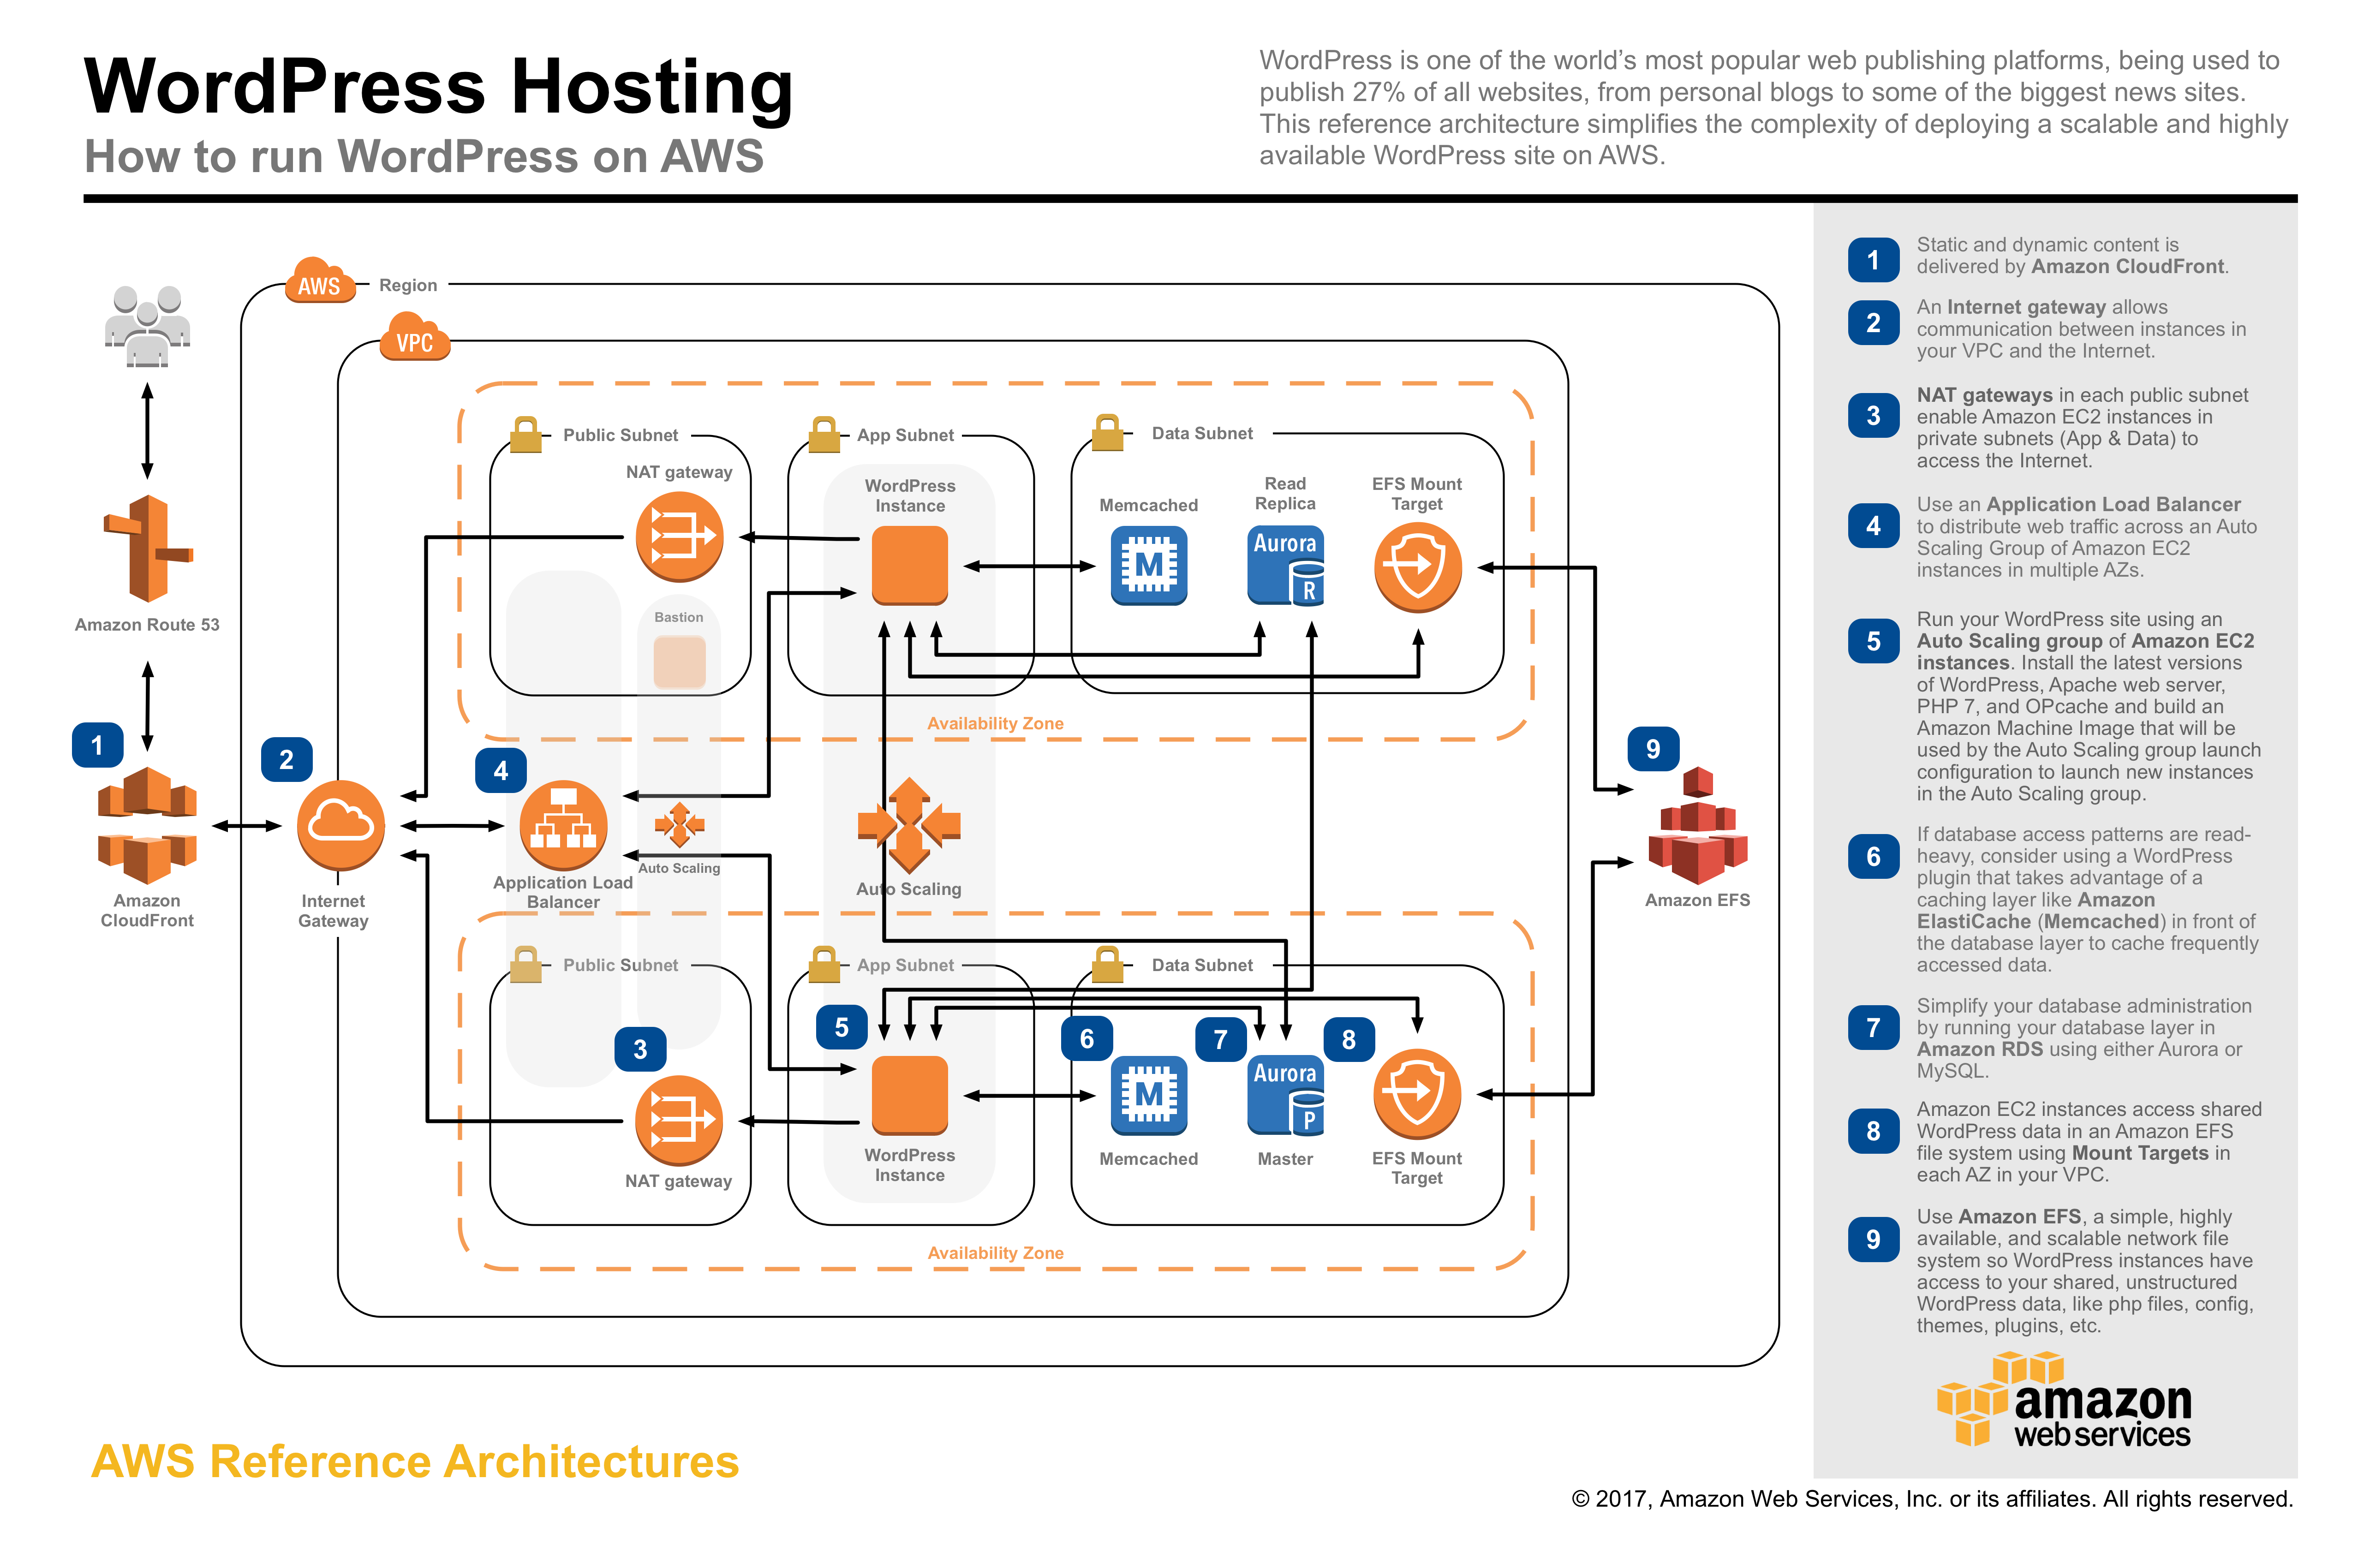
\includegraphics[width=\textwidth]{figs/AWS_Arquitecturas.jpeg}
		\caption{Arquitectura sugerida por AWS para una aplicaci�n en WordPress. Adaptado de \citep{AwsArchitectureSample}}\label{Arquitectura sugerida por AWS para una aplicaci�n en WordPress}
	\end{figure}
\end{landscape}
\begin{landscape}
	\begin{figure}[H]
		\centering
		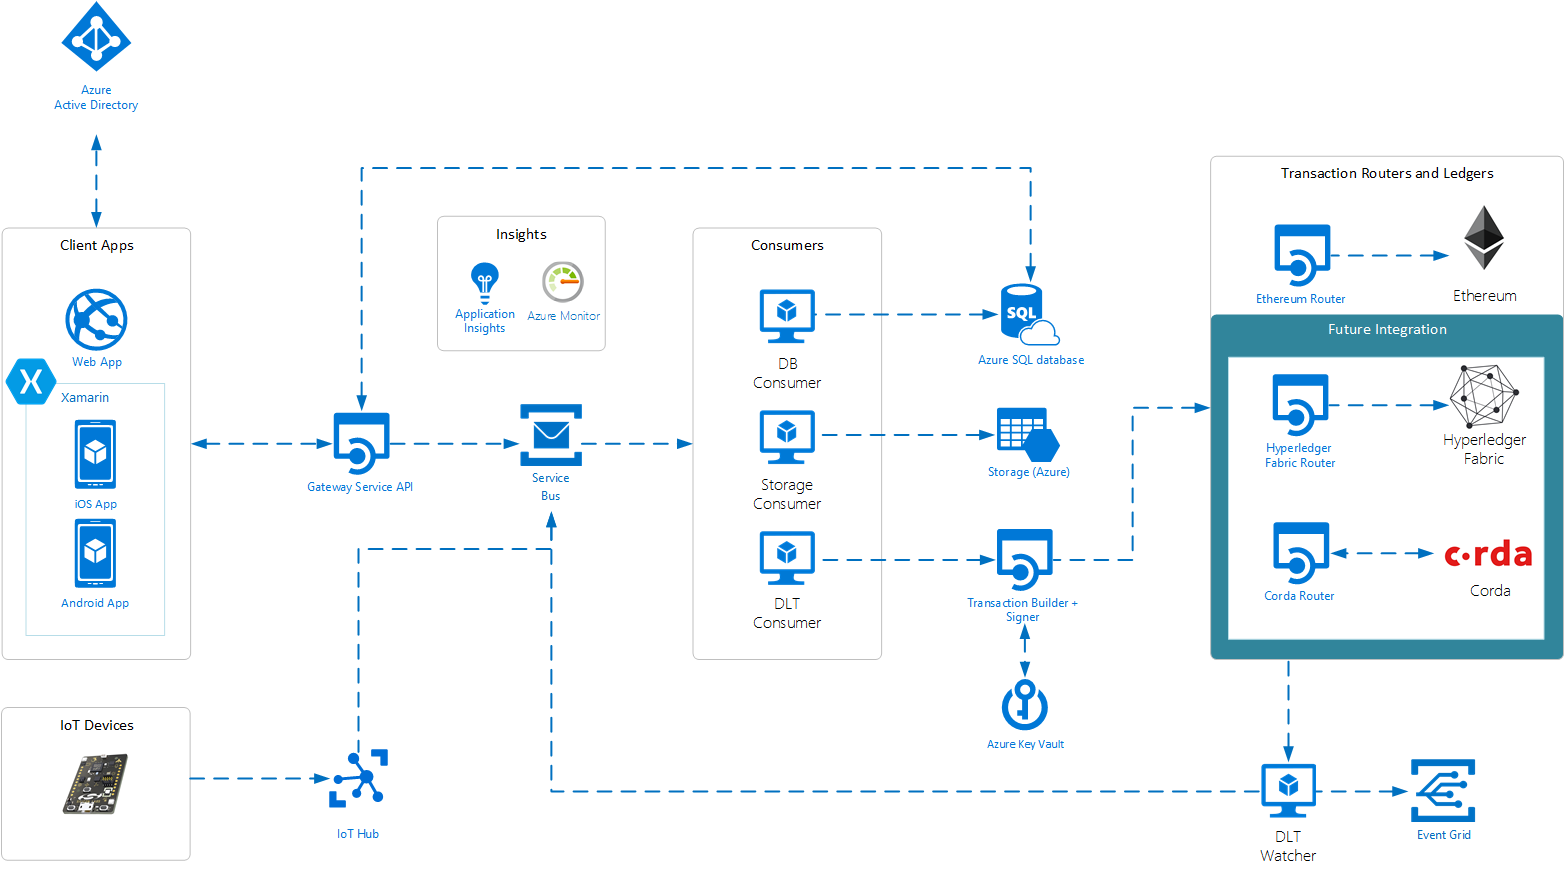
\includegraphics[width=\textwidth]{figs/AZURE_architecture.png}
		\caption{Arquitecturas sugeridas por Azure para una estaci�n de Blockchain. Adaptado de \citep{AzureArchitectureSample}}\label{Arquitecturas sugeridas por Azure para una estaci�n de Blockchain}
	\end{figure}
\end{landscape}
\begin{landscape}
	\begin{figure}[H]
		\centering
		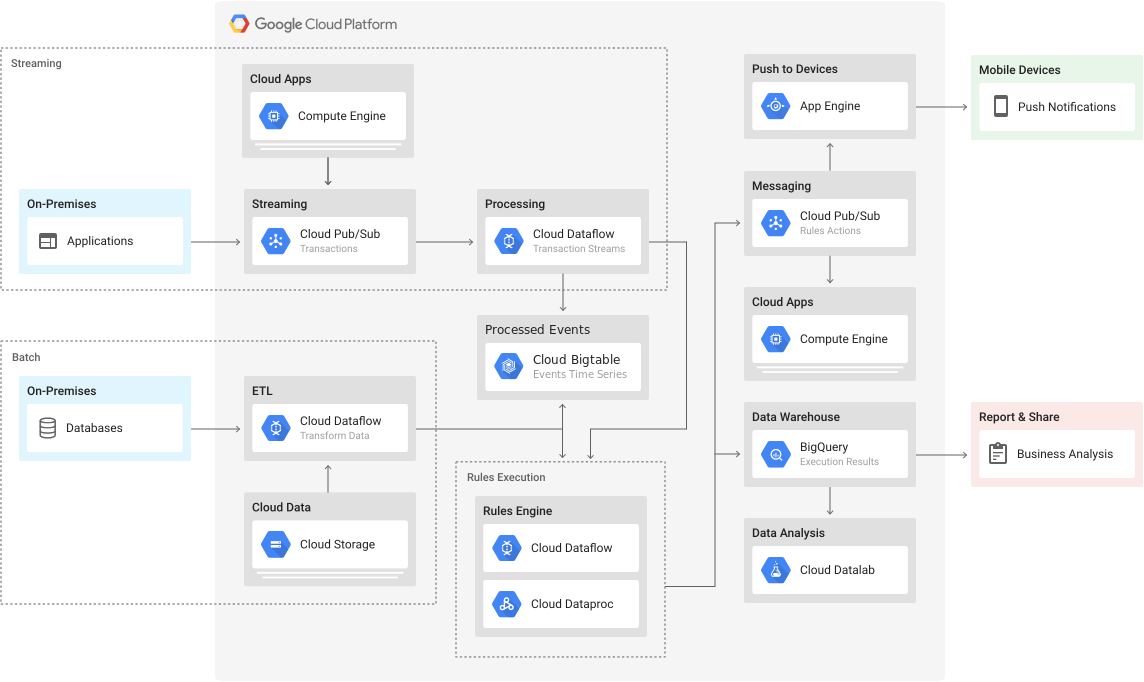
\includegraphics[width=\textwidth]{figs/GCP_architecture.png}
		\caption{Arquitecturas sugeridas por GCP para una aplicaci�n basada en eventos. Adaptado de \citep{GoogleArchitectureSample}}\label{Arquitecturas sugeridas por GCP para una aplicaci�n basada en eventos}
	\end{figure}
\end{landscape}   % Estado del arte

\chapter{Marco de referencia}
% ------------------------------------------------------------------------
\noindent En el presente Cap�tulo se presentan los conceptos b�sicos que ser�n abordados en Cap�tulos posteriores. 
% ------------------------------------------------------------------------

\section{Computaci�n en la nube}
Es un modelo para permitir el acceso, de manera extensa, conveniente y bajo demanda, a un grupo compartido de recursos inform�ticos configurables (Por ejemplo redes, servidores, almacenamiento, aplicaciones y servicios) que pueden provisionarse y lanzarse r�pidamente con un m�nimo esfuerzo administrativo o la interacci�n del proveedor de servicios \citep{MELL2011}.

\subsection{Caracter\'isticas esenciales}
\begin{itemize}
	\item {\textbf{Autoservicio sobre demanda:}} Los usuarios tienen acceso a recursos en la nube, por ejemplo capacidad de c�mputo o almacenamiento, bajo demanda siempre que sean necesarios.
	\item {\textbf{Amplio acceso a la red:}} Los recursos est�n disponibles a trav�s de la red y se accede por medio del mecanismo est�ndar que promueve el uso de la plataforma por un grupo variado de dispositivos cliente (Tel�fonos m�viles, tablets, laptops y estaciones de trabajo).
	\item {\textbf{Agrupaci�n de recursos:}} Es una abstracci�n sobre la manera en la cual se separa la manera en la cual se encuentran los recursos f�sicamente distribuidos y la asignaci�n de los mismo para los diferentes clientes. Los clientes suelen tener especificar la ubicaci�n de los recursos a un nivel alto de abstracci�n (por ejemplo, pa�s, estado o datacenter).
	\item {\textbf{Elasticidad:}} La capacidad de aumentar o disminuir los recursos asignados para poder escalar de la manera mas �ptima una aplicaci�n. Esto puede ser manual o autom�tico.
	\item {\textbf{Servicio medido:}} Los sistemas cloud poseen diferentes herramientas para poder medir el uso que se le da a los recursos asignados. Estas interfaces pueden ser gr�ficas o por l�nea de comando.
\end{itemize}

\subsection{Modelos de servicio}

\begin{itemize}
	\item {\textbf{Software como servicio:}} El cliente tiene acceso a una o varias aplicaciones que se encuentren ejecutando en la infraestructura cloud. El cliente se encuentra limitado al alcance que le provea la aplicaci�n.
	\item {\textbf{Plataforma como servicio:}} El cliente puede desplegar aplicaciones en la infraestructura cloud siempre que se usen tecnolog�as, como lenguajes de programaci�n, librer�as, servicios y herramientas, soportadas por el proveedor del servicio.
	\item {\textbf{infraestructura como servicio:}} El cliente puede desplegar y correr software de forma arbitraria, esto incluye sistema operativo y aplicaciones, por lo cual no se ve limitado a ninguna configuraci�n preliminar a nivel software.
\end{itemize}

En la figura \ref{Responsabilidades seg�n el modelo de servicio} se puede ver las responsabilidades del cliente y proveedor seg�n el modelo de servicio.

\begin{figure}[H]
	\centering
	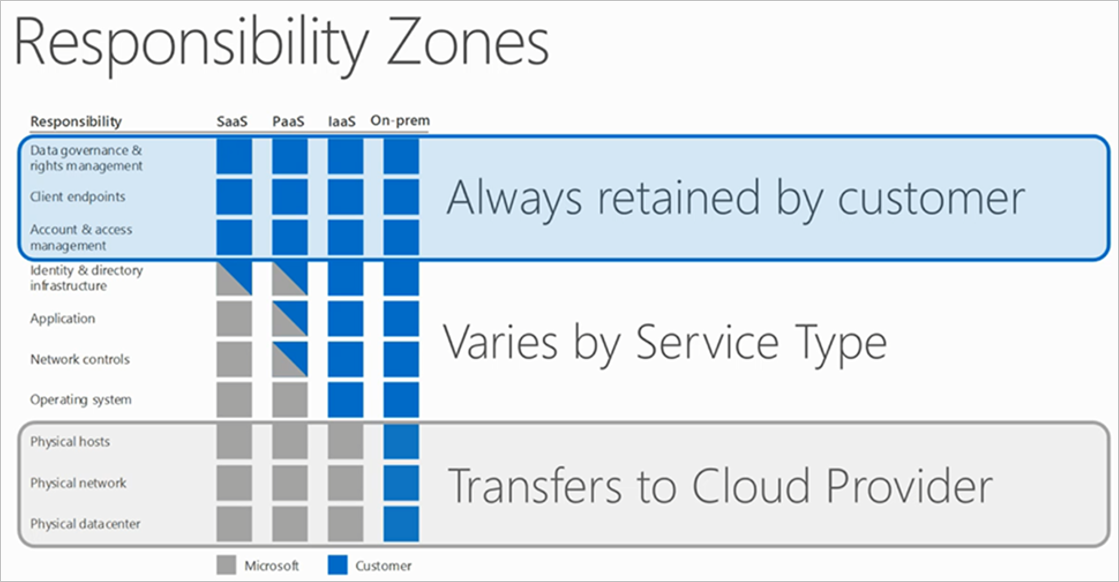
\includegraphics[width=\textwidth]{figs/responsibility-zones.png}
	\caption{Responsabilidades seg�n el modelo de servicio. Adaptado de \citep{GANTENBEIN2017}}\label{Responsabilidades seg�n el modelo de servicio}
\end{figure}


\subsection{Modelos de despliegue}
\begin{itemize}
	\item {\textbf{Nube privada:}} La infraestructura cloud es prove�da para el uso exclusivo de una organizaci�n. Puede ser propiedad, administrada y operada por la organizaci�n, un tercero o una combinaci�n de estos dos.
	\item {\textbf{Nube comunitaria:}} La infraestructura cloud es prove�da por una organizaci�n para el uso exclusivo de una comunidad de consumidores que tienen unas necesidades comunes.
	\item {\textbf{Nube p�blica:}} La infraestructura cloud es prove�da para el uso abierto de un p�blico general. Est� es administrada, operada y pose�da por una empresa, acad�micos, una organizaci�n del gobierno o una combinaci�n de los anteriores.
	\item {\textbf{Nube h�brida:}} La infraestructura cloud es una mezcla de dos o m�s tipos de infraestructura(Privada, comunitaria o p�blica).
\end{itemize}

\section{Alta disponibilidad}
En computaci�n, disponibilidad es la capacidad de un m�dulo para ejecutar una funci�n cuando se es requerido. La disponibilidad se expresa de la siguiente manera:

\begin{equation}
Disponibilidad = \dfrac{Tiempo de servicio - Tiempo de inactividad}{Tiempo de servicio} * 100
\end{equation}

Cuando hablamos de ?Alta disponibilidad?, hacemos referencia a que cumple el m�ximo est�ndar: la disponibilidad medida es de 99.999\% \citep{BENZ2013}.

El objetivo de la alta disponibilidad es eliminar los puntos de fallo potencial en la infraestructura. Un punto de fallo potencial es un componente del stack tecnol�gico que puede producir una interrupci�n del sistema. Al igual, todo componente que sea necesario para el sistema y no tenga redundancia, tambi�n se considera un punto de falla \citep{HEIDI2016}.

Existen 2 tipos de cluster de alta disponibilidad: \citep{VILLANUEVA2015}

\begin{itemize}
	\item {\textbf{Activo-Activo:}} Se suelen tener al menos 2 nodos, ambos se encuentran corriendo la misma clase de servicios de manera simult�nea. El prop�sito principal de un cluster con alta disponibilidad de tipo activo-activo es lograr un buen balanceo de carga. El balanceo de cargas distribuye las solicitudes sobre todos los nodos con el fin de evitar que un solo nodo se sobrecargue. La configuraci�n m�s sencilla es presentada en la figura \ref{Modelo de un cluster activo-activo}
	
		\begin{figure}[H]
			\centering
			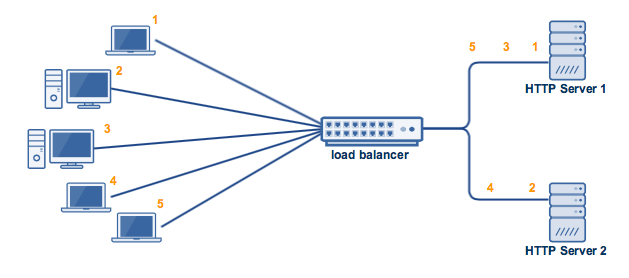
\includegraphics[width=\textwidth]{figs/active_active_high_availability_cluster_load_balancer.png}
			\caption{Modelo de un cluster activo-activo. Adaptado de \citep{VILLANUEVA2015}}\label{Modelo de un cluster activo-activo}
		\end{figure}
		
		Este modelo tiene un balanceador de carga y 2 servidores http. Los clientes no se conecta directamente a los servidores http, sino que las solicitudes pasan por medio de un balanceador de carga, el cual usa un algoritmo para determinar a qu� servidor se direccionan las solicitudes.
		
		Este modelo se recomienda para aplicaciones que van a tener una cantidad masiva de conexiones durante un tiempo prolongado.
		
		\item {\textbf{Activo-Pasivo:}} Al igual que la configuraci�n activo-activo, la configuraci�n activo-pasivo requiere al menos de 2 nodos. Se conoce como activo-pasivo por que no todos los nodos empiezan activos. 
		
		El nodo pasivo es un respaldo cuya funci�n es recibir las solicitudes de los clientes tan pronto como el nodo activo se desconecte o quede inhabilitado para poder responder a las solicitudes de los usuarios. En la figura \ref{Modelo de un cluster activo-pasivo} se presenta este modelo.
		
		\begin{figure}[H]
			\centering
			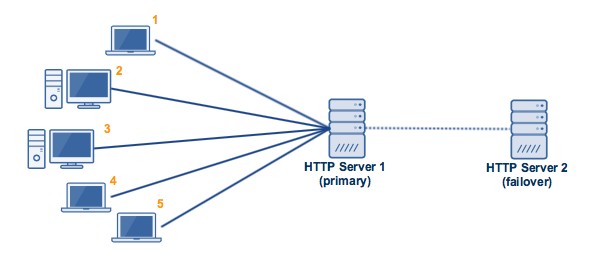
\includegraphics[width=\textwidth]{figs/active_passive_high_availability_cluster.png}
			\caption{Modelo de un cluster activo-pasivo. Adaptado de \citep{VILLANUEVA2015}}\label{Modelo de un cluster activo-pasivo}
		\end{figure}
			
		Est� configuraci�n se recomienda cuando no se va a tener que lidiar con una cantidad masiva de solicitudes durante un tiempo prolongado pero existen escenarios en los cuales la cantidad de peticiones puede aumentar de manera considerable.
\end{itemize}
		
\subsection{Escalabilidad}
Escalabilidad es la capacidad que tiene una soluci�n para poder adaptarse al crecimiento en la demanda.

Imaginemos que tenemos una aplicaci�n corriendo en un servidor con ciertas caracter�sticas, de repente la cantidad de usuarios de nuestra aplicaci�n aumenta por lo cual se hace necesario escalar nuestra infraestructura con el fin de poder seguir brindando el mejor servicio. Existen 2 maneras de escalar:

\begin{itemize}
	\item {\textbf{Escalabilidad vertical:}} Era la forma de escalar convencional hace unos a�os y es b�sicamente aumentar las capacidades del equipo de computo o en su defecto, comprar uno nuevo con m�s capacidad. Es la forma m�s sencilla de escalar ya que ya que la arquitectura de la infraestructura no cambia.
	\item {\textbf{Escalabilidad horizontal:}} Consiste en distribuir la carga en un conjunto de equipos de c�mputo, de tal manera que si necesitamos soportar una mayor carga, en lugar de cambiar todo el hardware por uno de mayor capacidad, lo que usualmente es muy costoso, simplemente a�adimos un nuevo equipo al conjunto lo cual implica una redistribuci�n de la carga y aumenta la cantidad que el conjunto puede llegar a soportar. 
\end{itemize}
\begin{figure}[H]
	\centering
	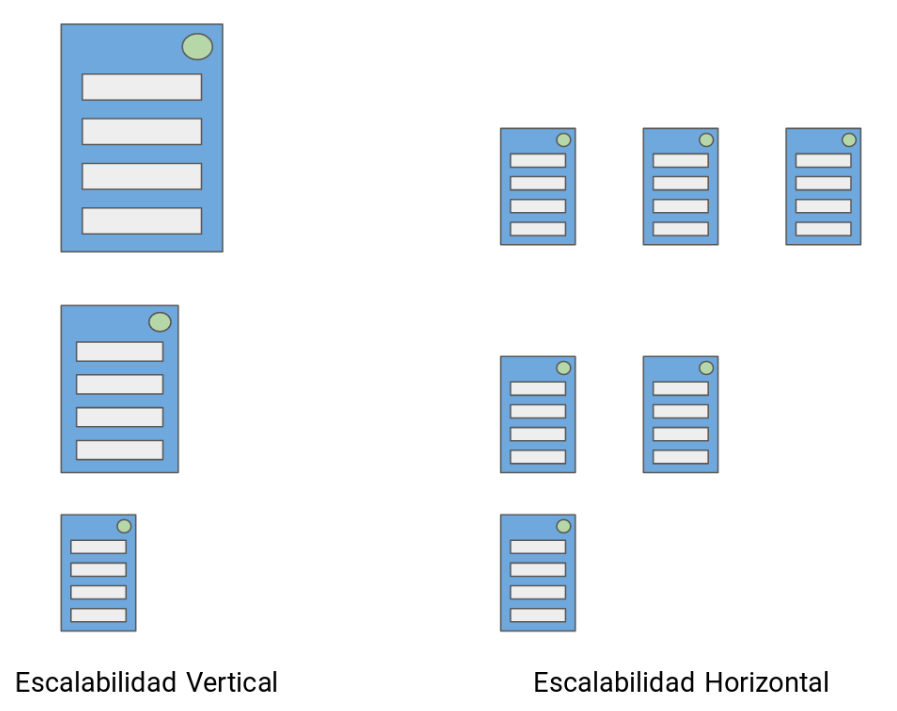
\includegraphics[width=0.8\textwidth]{figs/escalabilidad.png}
	\caption{Escalabilidad vertical en contraste con escalabilidad horizontal.}\label{Escalabilidad vertical en contraste con escalabilidad horizontal}
\end{figure}

La escalabilidad vertical tiene un problema: La ley de Moore, la cual dicta: ?Cada dos a�os, aunque en principio dijo que ser�a cada 18 meses, se duplica el n�mero de transistores. Seg�n la sia, aunque es f�sicamente posible que los fabricantes de microprocesadores lleguen a crear algunos chips m�s de lo estipulado por Moore, no ser�a pr�ctico a nivel financiero, debido a los altos costos que implica.

"Y, siendo optimistas, la fecha l�mite, de acuerdo con el presidente y CEO de la sia John Neuffer ser�a, como mucho, 2030 \citep{BBC2018}. En otras palabras, va a llegar un punto en el cual, aunque tengamos dinero ilimitado para poder comprar el equipo de computo mas poderoso en el mercado, va llegar un punto donde el equipo que pueda satisfacer nuestra demanda no exista, lo cual convierte la escalabilidad vertical en una soluci�n inviable para aplicaciones que visionan un crecimiento masivo.

Por otra parte, la escalabilidad horizontal, a pesar de ser m�s compleja compleja en t�rminos de arquitectura, puede escalar sin estar limitada por la ley de Moore adem�s que, al tener la carga distribuida en varios nodos, podemos proveer un servicio de alta disponibilidad y los costos para escalar

\section{Virtualizaci\'on}
La virtualizaci�n es una capa intermedia a nivel de sistema operativo que provee una abstracci�n de los recursos del sistema. Es tal el papel de la virtualizaci�n dentro del cloud computing que grandes compa��as, como Amazon, Google y Microsoft, basan sus servicios cloud en la virtualizaci�n.

Las m�quinas virtuales son impulsadas por los hipervisores. El hipervisor es un software que provee un entorno aislado para cada m�quina virtual y es responsable de correr diferentes kernels a nivel del sistema operativo anfitri�n.

\begin{figure}[H]
	\centering
	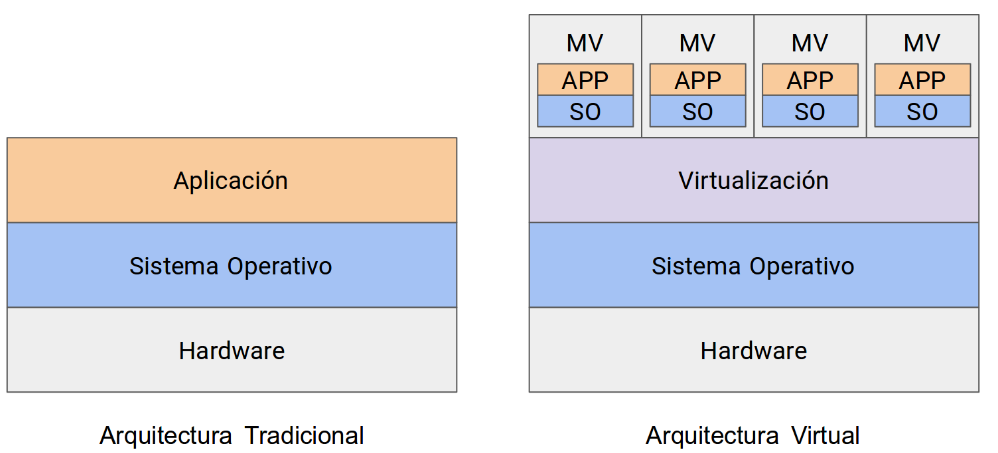
\includegraphics[width=\textwidth]{figs/virtualizacion.png}
	\caption{Arquitectura tradicional en contraste con arquitectura con m�quinas virtuales.}\label{Arquitectura tradicional en contraste con arquitectura con m�quinas virtuales}
\end{figure}

Como podemos ver en la figura \ref{Arquitectura tradicional en contraste con arquitectura con m�quinas virtuales}, en la arquitectura tradicional hay un acceso m�s directo al hardware pero posee las siguientes falencias:

\begin{itemize}
	\item Solo se pueden ejecutar aplicaciones de un sistema operativo.
	\item Las aplicaciones no se corren en un ambiente aislado por lo que un fallo en el sistema afecta directamente a todas las aplicaciones.
	\item No hay portabilidad en las aplicaciones.
\end{itemize}

Las m�quinas virtuales resuelven los problemas anteriormente mencionados usando el hipervisor, el cual nos permite crear m�quinas virtuales con diferentes sistemas operativos corriendo al tiempo por lo que podemos tener corriendo, en una misma m�quina, aplicaciones para Linux y para Windows al tiempo, adicionalmente cada aplicaci�n puede estar corriendo en ambientes aislados por lo que un fallo en una aplicaci�n no va a afectar a las dem�s aplicaciones. Sin embargo, las m�quinas virtuales tienen los siguientes problemas:

\begin{itemize}
	\item Los recursos necesarios es significativamente mayor al enfoque tradicional debido a que se deben correr los servicios de cada sistema operativo adicional por cada m�quina virtual.
	\item El rendimiento de las aplicaciones dentro de las m�quinas virtuales se ve afectado.
	\item Los tiempos de encendido y apagado de las m�quinas virtuales pueden llegar a ser del orden de minutos.
\end{itemize}

Para solucionar estos problemas aparecen los contenedores.

\section{Contenedores}

Las aplicaciones software suelen desplegarse como un conjunto de librer�as y archivos de configuraci�n en un entorno, por ejemplo, un servidor. Estas se despliegan en un sistema operativo con un conjunto de servicios corriendo, como puede ser un servidor de base de datos o un servidor http, sin embargo estos servicios pueden ser desplegados en cualquier ambiente que pueda proveer los mismos servicios, ya sea una m�quina virtual o una m�quina f�sica. 

Sin embargo, esta metodolog�a tiene un problema relacionado con la actualizaci�n o parches ya que estos pueden, por problemas de compatibilidad, dejar una aplicaci�n fuera de servicio. Otro escenario es el cual tenemos 2 aplicaciones en un mismo sistema operativo anfitri�n las cuales comparten librer�as, luego para solucionar un problema con la aplicaci�n 1, surge la necesidad de actualizar una de las librer�as, en cuyo caso se corre el riesgo de afectar el funcionamiento de la aplicaci�n 2. Para poder evitar cualquier inconveniente durante el despliegue, las compa��as de software suelen hacer pruebas antes de realizar el despliegue en el sistema de producci�n, sin embargo, seg�n la complejidad de la aplicaci�n, estas pruebas pueden llegar a ser una tarea tediosa.

\begin{figure}[H]
	\centering
	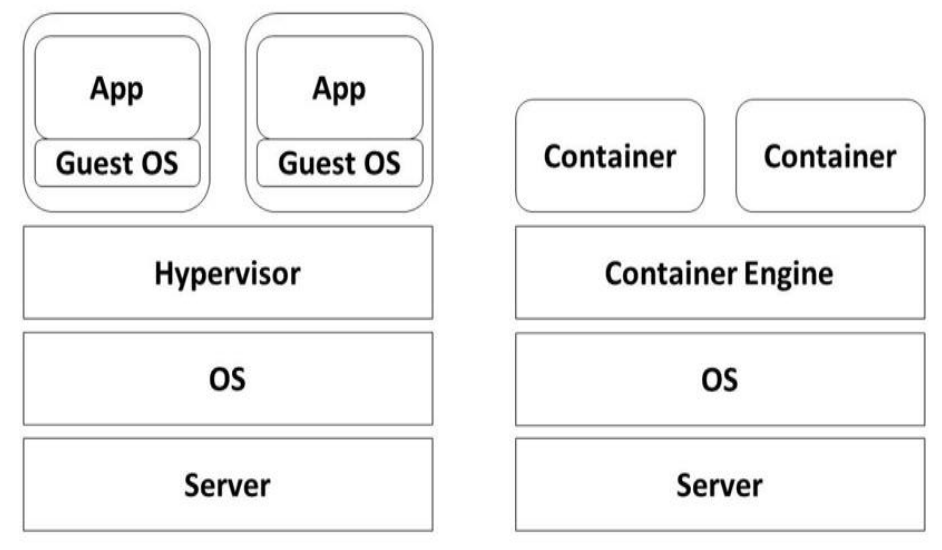
\includegraphics[width=\textwidth]{figs/contenedores.png}
	\caption{M�quinas virtuales vs contenedores. Adaptado de \citep{JOY2015}}\label{M�quinas virtuales vs contenedores}
\end{figure}

Como alternativa, aparecen los contenedores los cuales son un ambiente aislado dentro de un sistema operativo. Los contenedores toman ciertos beneficios de las m�quinas virtuales, como la seguridad, el almacenamiento y el aislamiento de red, mientras que consumen muchos menos recursos que las m�quinas virtuales. Adicionalmente, los contenedores nos proveen un rendimiento y escalabilidad mayor a las m�quinas virtuales como se muestra en la figura \ref{Solicitudes procesadas en 600 segundos}


\begin{figure}[H]
	\centering
	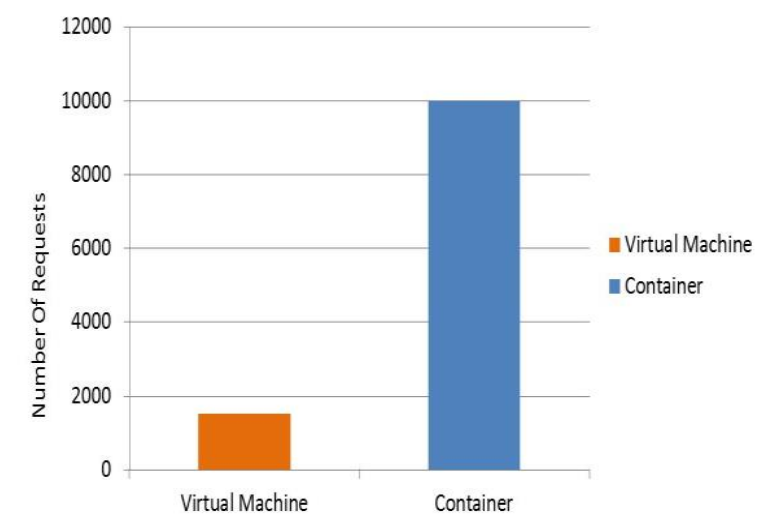
\includegraphics[width=\textwidth]{figs/solicitudes.png}
	\caption{Solicitudes procesadas en 600 segundos. Adaptado de \citep{JOY2015}}\label{Solicitudes procesadas en 600 segundos}
\end{figure}

Los contenedores poseen las siguientes ventajas:

\begin{itemize}
	\item Poco impacto sobre los recursos
	\item Ambiente aislado
	\item Despliegue r�pido
	\item Portabilidad
\end{itemize}

\section{Orquestaci\'on de contenedores}

Supongamos que tenemos una aplicaci�n desplegada usando contenedores y por alguna raz�n, ya sea un ataque por denegaci�n de servicios o un simple error en el c�digo de la aplicaci�n, el contenedor que la contiene falla. En un sistema de disponibilidad alta debemos asegurar de alguna manera que la aplicaci�n siempre va a estar disponible, por lo tanto debemos implementar una arquitectura que nos permita tolerar fallos, es aqu� donde aparece el siguiente concepto: ?Orquestaci�n de contenedores?. 

La orquestaci�n de contenedores nos permite desplegar un nuevo contenedor en caso de que otro falle con el fin de mantener la consistencia dentro del cluster, gestionar la manera en que los diferentes contenedores interact�an entre s�. Existen varias tecnolog�as que implementan una arquitectura para orquestar contenedores: Kubernetes, Docker Swarm o Fleet.

\section{Microservicios}
Los microservicios son una arquitectura y un enfoque sobre la escritura de software en el que las aplicaciones se dividen en componentes m�s peque�os e independientes entre s�. A diferencia de un enfoque tradicional y monol�tico sobre las aplicaciones, en el que todo se crea en una �nica pieza, los microservicios est�n separados y funcionan conjuntamente para llevar a cabo las mismas tareas como podemos ver en la figura \ref{Arquitectura monol�tica vs arquitectura de microservicios}. Cada uno de estos componentes, o procesos, son los microservicios. Este enfoque sobre el desarrollo de software valora la granularidad por ser liviana y la capacidad de compartir un proceso similar en varias aplicaciones. \citep{WhatAreMicroservices}


\begin{figure}[H]
	\centering
	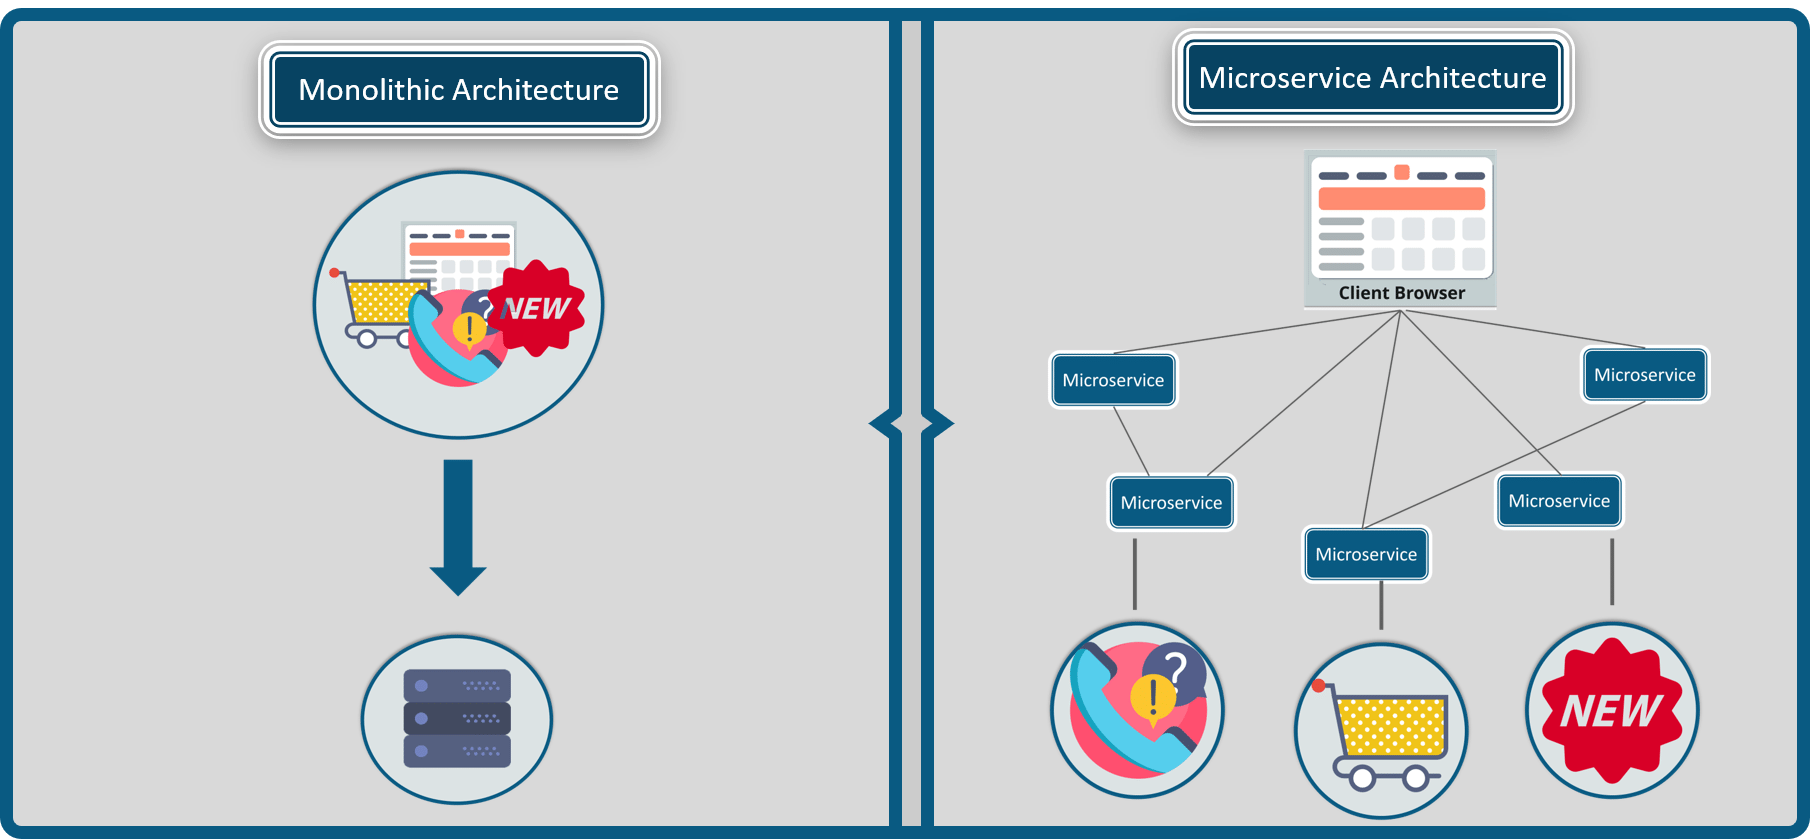
\includegraphics[width=\textwidth]{figs/monolithic-vs-microservices.png}
	\caption{Arquitectura monol�tica vs arquitectura de microservicios. Adaptado de \citep{EdurekaMicroservices}}\label{Arquitectura monol�tica vs arquitectura de microservicios}
\end{figure}   	% Marco de referencia
% ------------------------------------------------------------------------
% ------------------------------------------------------------------------
% ------------------------------------------------------------------------
%                                Cap�tulo 4
% ------------------------------------------------------------------------
% ------------------------------------------------------------------------
% ------------------------------------------------------------------------

\chapter{Marco t�cnico}
% ------------------------------------------------------------------------.
\noindent En este cap�tulo se abordaran las tecnolog�as usadas durante el proyecto para implementar los conceptos abordados en el Cap�tulo 3.
% ------------------------------------------------------------------------
% ------------------------------------------------------------------------
% ------------------------------------------------------------------------

\section{Docker}
Docker es una tecnolog�a de creaci�n y uso de contenedores Linux, para ello hace uso del kernel de Linux y funciones del mismo como Cgroups y namespaces para aislar procesos y que estos se puedan ejecutar de forma independiente. 

Docker ofrece un modelo de implementaci�n basado en im�genes lo cual permite compartir una aplicaci�n o conjunto de servicios, junto con sus dependencias en varios entornos. Adem�s, Docker automatiza la implementaci�n de la aplicaci�n (o conjuntos combinados de procesos que conforman una aplicaci�n) dentro del entorno del contenedor \citep{RHDocker}.

Del ecosistema Docker, se destacan los siguientes componentes:
\begin{itemize}
	\item\textbf{Contenedor:} Ambiente que permite ejecutar aplicaciones de manera aislada en un sistema anfitri�n. Son creados a partir de im�genes. Haciendo una analog�a con la programaci�n orientada a objetos, son las instancias de las im�genes, es decir, a partir de una imagen pueden crearse n contenedores con el mismo estado.
	\item\textbf{Imagen:} Template que describe el estado inicial de un contenedor. Una imagen puede ser construida a partir de otra imagen disponible en un registro remoto. Haciendo una analog�a con al programaci�n orientada a objetos, una imagen es una clase que puede ser instanciada n veces en forma de contenedor.
	\item\textbf{Registro:} Es un repositorio de im�genes. Puede ser p�blico o privado, es decir que es posible trabajar con im�genes disponibles en internet. Uno de los registros p�blicos mas populares es Docker Hub, el cual pertenece a Docker Inc.
\end{itemize}

\section{Kubernetes}

Es una plataforma open source que automatiza las operaciones de contenedores Linux. Elimina varios procesos en la implementaci�n y escalabilidad de las aplicaciones en contenedores, lo cual nos permite construir y administrar un cl�ster de contenedores de forma eficiente y sencilla. Los cl�ster pueden ser construidos en nubes p�blicas, privadas, comunitarias o h�bridas.


Un cluster Kubernetes es un conjunto de servidores que ejecutan diferentes servicios como podemos ver en la figura \ref{Arquitectura de un cluster Kubernetes} \citep{KubenetesComponentes}.

\begin{figure}[H]
	\centering
	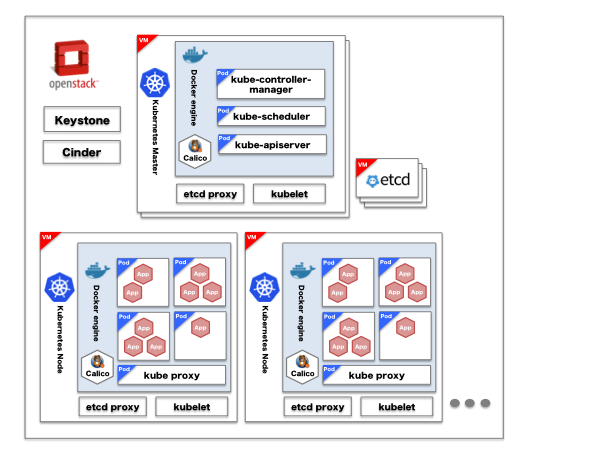
\includegraphics[width=\textwidth]{figs/arquitectura_kubernetes.png}
	\caption{Arquitectura de un cluster Kubernetes. Adaptado de \citep{KubenetesArquitectura}}\label{Arquitectura de un cluster Kubernetes}
\end{figure}

\section{Objetos Kubernetes}
Los objetos Kubernetes son entidades que persisten dentro del sistema Kubernetes. Kubernetes usa estas entidades para representar el estado del cluster, para ello se definen en archivos en formato YAML o JSON. Espec�ficamente, los objetos Kubernetes describen \citep{KubenetesObjetos}:

\begin{itemize}
	\item Que aplicaciones se encuentran en ejecuci�n.
	\item Los recursos disponibles para cada aplicaci�n en ejecuci�n.
	\item Las pol�ticas del cluster. 
\end{itemize}

El conjunto de objetos Kubernetes dentro del cluster define el estado deseado del cluster y Kubernetes se encargar� de monitorear y gestionar los diferentes nodos con el fin de que el estado del cluster sea igual al estado deseado del mismo. 

\begin{itemize}
	\item \textbf{Pod:} Conjunto de contenedores. El pod es la unidad m�nima en Kubernetes.
	\item \textbf{Service:} Interfase entre cliente y la aplicaci�n dentro de los pods. Es una pareja ip-puerto est�tica que se encarga de redirigir las solicitudes entre los diferentes pods disponibles.
	\item \textbf{Persistent Volumes:} Permite definir un sistema de almacenamiento dentro del cluster.
	\item \textbf{Persistent Volumes Claims:} Representa una solicitud para obtener recursos de almacenamiento del cluster.
\end{itemize}

\section{Openshift}
Openshift es un PaaS ofrecido por Red Hat con una integraci�n nativa con Docker y Kubernetes, a�adiendo funcionalidades de las cuales Kubernetes carece como:
\begin{itemize}
	\item Integraci�n con herramientas de integraci�n continua como Jenkins.
	\item Manejo de diferentes proyectos en un mismo cluster.
	\item Plantillas que facilitan el despliegue de aplicaciones.
\end{itemize}


\begin{figure}[H]
	\centering
	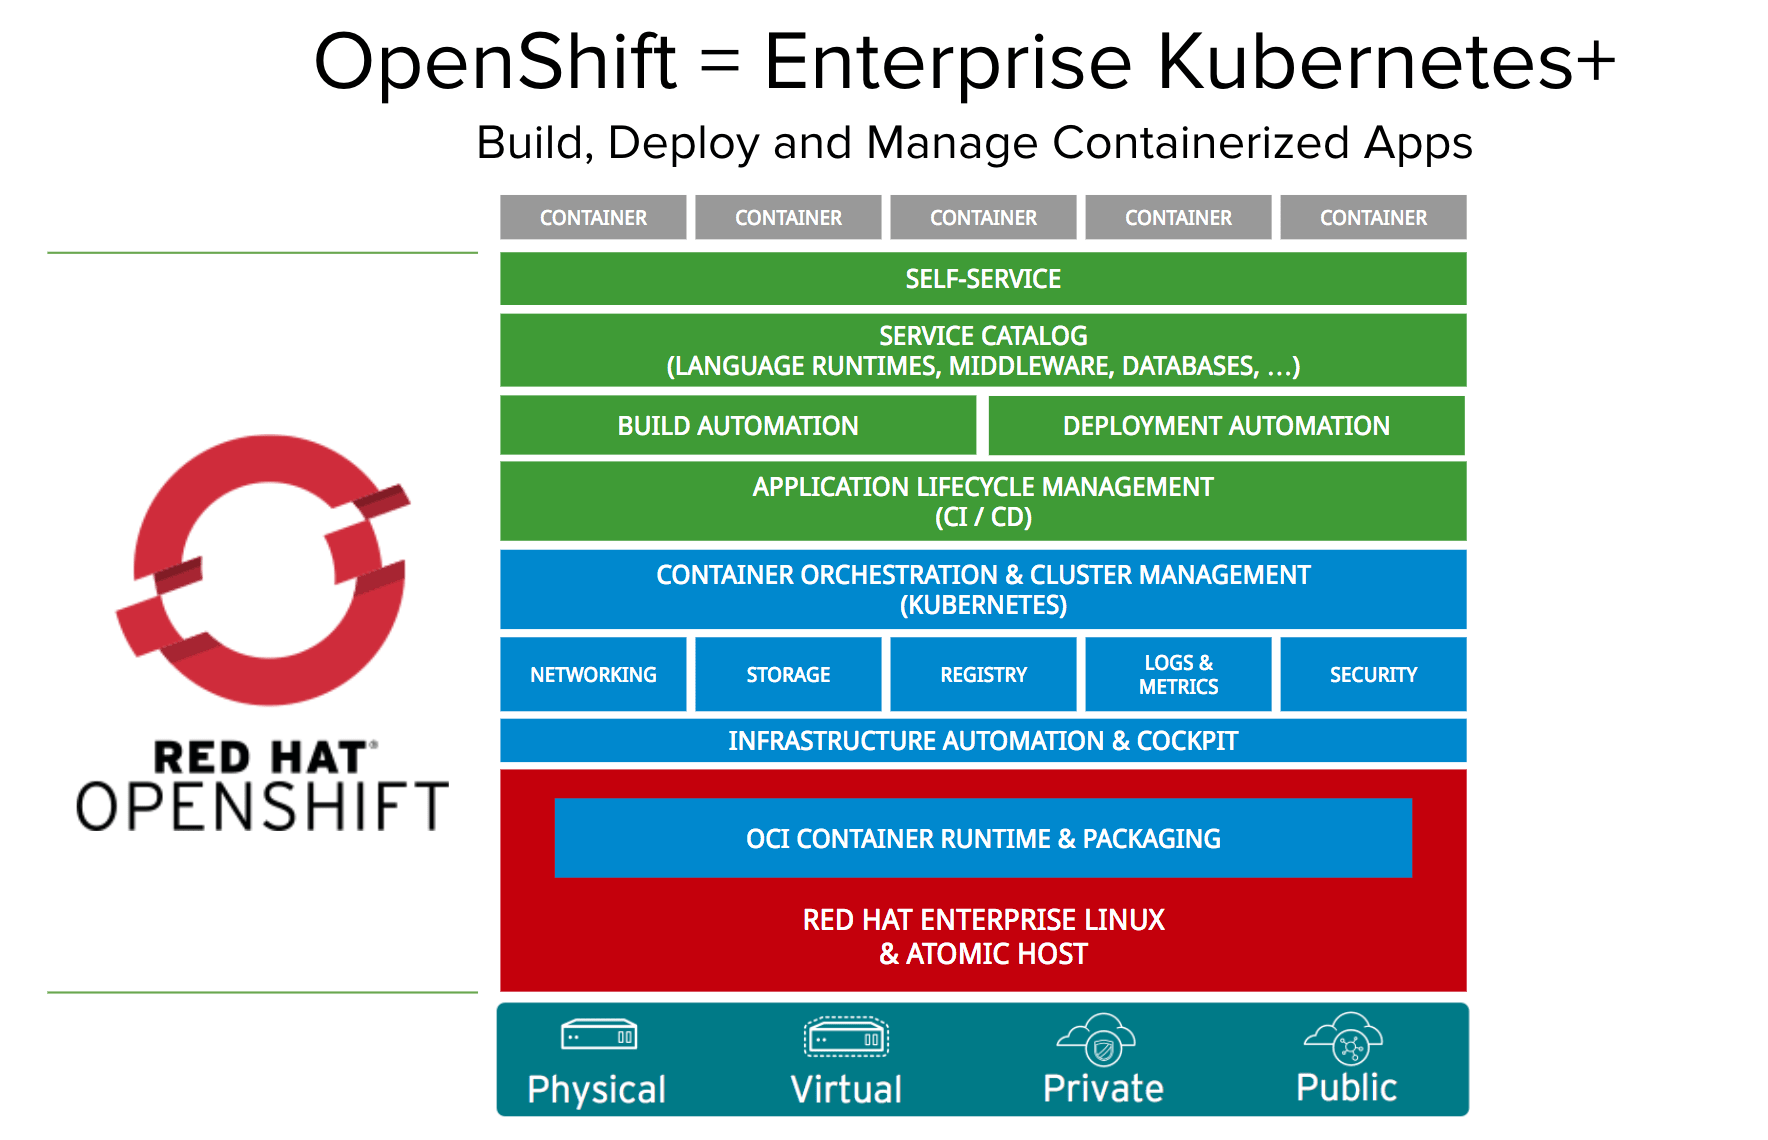
\includegraphics[width=\textwidth]{figs/OpenShiftContainerPlatformStack.png}
	\caption{Arquitectura de Openshift. Adaptado de \citep{OpenshiftArquitectura}}\label{Arquitectura de Openshift}
\end{figure}


\section{Ansible}
Ansible es una herramienta para automatizar la administraci�n de una infraestructura TI por medio de archivos de configuraci�n llamados Ansible Playbooks en los cuales se describen los diversos pasos a automatizar\citep{ansibledocumentation}.

En la arquitectura de Ansible, se tiene un archivo YAML, llamado Inventory, en el cual se describen los diferentes elementos de la infraestructura TI y variables de configuraci�n. Posteriormente se ejecutan los playbooks usando el Inventory y Ansible indica si el proceso fue ejecutado con exito o hubo alg�n problema durante alguno de los pasos del playbook.

\section{GlusterFS}
GlusterFS es un sistema de archivos en red escalable dise�ado para tareas de alto uso de datos como almacenamiento cloud \citep{glusterfs}.

\begin{itemize}
	\item {\textbf{Sistema de archivo en red}} Es un sistema de archivos que distribuye los datos en diferentes nodos.
	\item {\textbf{Brick}} Es cualquier directorio o partici�n que es asignado a formar parte de un volumen.
	\item {\textbf{Volumen}} Es un conjunto l�gico de Bricks. Las operaciones se basan en los diferentes tipos de vol�menes creados por el usuario.
\end{itemize}

\begin{figure}[H]
	\centering
	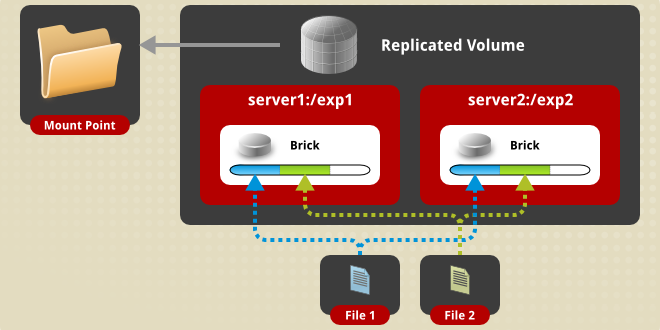
\includegraphics[width=0.75\textwidth]{figs/glusterfs.png}
	\caption{Arquitectura de Glusterfs. Adaptado de \citep{glusterfs}}\label{Arquitectura de Glusterfs}
\end{figure}
   	% Marco t�cnico
% ------------------------------------------------------------------------
% ------------------------------------------------------------------------
% ------------------------------------------------------------------------
%                            Recomendaciones
% ------------------------------------------------------------------------
% ------------------------------------------------------------------------
% ------------------------------------------------------------------------

\chapter{Desarrollo del proyecto}
% ------------------------------------------------------------------------
\noindent En este Cap�tulo se presentar� como fue desarrollado el proyecto.
% ------------------------------------------------------------------------ 
\section{Ambientaci�n tecnol�gica}
\subsection{Investigaci\'on fundamentos te\'oricos relacionados con el proyecto (Tecnolog\'ias y est\'andares)}
Durante esta primera fase se investig� el estado del arte en cloud computing para poder identificar los conceptos comunes en las diferentes arquitecturas cloud enfocadas a IoT. De esta primera fase se encontr� la gesti�n de contenedores como factor com�n por lo cual la investigaci�n posterior sigui� este enfoque. Posteriormente se identificaron las tecnolog�as m�s populares en IoT.

\begin{table}[H]
	\begin{minipage}{1\textwidth}
		\caption[Tecnolog�as disponibles en el mercado]{ \raggedright Tecnolog�as disponibles en el mercado}
		\label{tabla:Tecnolog�as disponibles en el mercado}
		\begin{center}
			\begin{tabular}{ p{5cm}   p{5cm}  p{5cm}  }
				\hline
				Sistema Operativo & Container Runtime & Orquestador de contenedores \\
				\hline
				CentOS & Cri-O & Apache Mesos \\
				CoreOS & Docker & Docker Swarm \\
				Red Hat Enterprise Linux & Linux VServer & Kontena \\
				Oracle Linux & LXD & Kubernetes \\
				Ubuntu Server & Rkt  & Nomad \\
				Windows Server & Windows Containers & Openstack Magnum x
				\\ \hline
			\end{tabular}
		\end{center}
	\end{minipage}
\end{table}

A medida que se desarroll� en proyecto, nuevas tecnolog�as fueron a�adidas al stack pero ya de eso se hablar� m�s adelante en el documento.

A medida que se desarroll� en proyecto, nuevas tecnolog�as fueron a�adidas al stack pero ya de eso se hablar� m�s adelante en el documento.

\subsection{Estudio}
Durante esta etapa se realiz� una revisi�n general sobre cada una de las tecnolog�as, lo cual sirvi� de base para la definir los criterios de selecci�n para realizar un primer filtro sobre las tecnolog�as a usar en la infraestructura en la siguiente etapa.

\begin{itemize}
	\item Licencia
	\item Stacks
	\item Soporte
	\item Uso libre en producci�n
\end{itemize}



\subsection{Sondeo}
Durante esta etapa se aplicaron los diferentes criterios entre cada una de las tecnolog�as y se consolido est� informaci�n en las tablas \ref{tabla:Sondeo de selecci�n: Sistema Operativo}, \ref{tabla:Sondeo de selecci�n: Container Runtime} y \ref{tabla:Sondeo de selecci�n: Orquestador de contenedores}.
\begin{table}[H]
	\begin{minipage}{1\textwidth}
		\caption[Sondeo de selecci�n: Sistema Operativo]{ \raggedright Sondeo de selecci�n: Sistema Operativo}
		\label{tabla:Sondeo de selecci�n: Sistema Operativo}
		\begin{center}
			\begin{tabular}{ p{3cm}   p{3cm}  p{2cm}  p{3cm}  p{4cm}  }
				\hline
				S. Operativo & Licencia & Stacks & Soporte & Gratis en producci�n \\  \hline
				CentOS & GPL & 1.85K & Comunidad & Si
				\\ 
				CoreOS & Apache 2.0 & 164 & Comunidad & Si
				\\ 
				RHEL\footnote{Red Hat Enterprise Linux} & GPL\footnote{Solo para efectos de desarrollo, en producci�n se cobra una tarifa.} & - & Privado & No
				\\ 
				Oracle Linux & GPL & - & Privado & Si
				\\ 
				Ubuntu Server & GPL & 9.1k & Hibrido\footnote{Posibilidad de adquirir soporte pago pero posee una gran comunidad que lo respalda.} & Si
				\\ 
				Windows Server & M�ltiple\footnote{Microsoft provee diferentes licencias seg�n los servicios solicitados.} & 3.4k & Privado & No
				\\ \hline
			\end{tabular}
		\end{center}
		{La cantidad de stacks fueron tomados de: \url{https://stackshare.io/}}
	\end{minipage}
\end{table}


\begin{table}[H]
	\begin{minipage}{1\textwidth}
		\caption[Sondeo de selecci�n: Container Runtime]{ \raggedright Sondeo de selecci�n: Container Runtime}
		\label{tabla:Sondeo de selecci�n: Container Runtime}
		\begin{center}
			\begin{tabular}{ p{3cm}  p{3cm} p{2cm}  p{4cm}  p{3cm}  }
				\hline
				Container Runtime & Licencia & Stacks & Soporte & Uso libre en producci�n \\ \hline
				Cri-O & Apache 2.0 & - & Comunidad & Si
				\\ 
				Docker & Apache 2.0 & 16.6K & Comunidad/Privado & Si
				\\ 
				Linux VServer & GPL & - & Comunidad & Si
				\\ 
				LXD & Apache 2.0 & 39 & Comunidad & Si
				\\ 
				Rkt & Apache 2.0 & 21 & Comunidad & Si
				\\
				Windows Containers & SaaS & - & Privado & No
				\\ \hline
			\end{tabular}
		\end{center}
		{La cantidad de stacks fueron tomados de:
			\url{https://stackshare.io/}}
	\end{minipage}
\end{table}


\begin{table}[H]
	\begin{minipage}{1\textwidth}
		\caption[Sondeo de selecci�n: Orquestador de contenedores]{ \raggedright Sondeo de selecci�n: Orquestador de contenedores}
		\label{tabla:Sondeo de selecci�n: Orquestador de contenedores}
		\begin{center}
			\begin{tabular}{ p{3cm}   p{3cm}  p{2cm}  p{4cm}  p{3cm}  }
				\hline
				Orquestador & Licencia & Stacks & Soporte & Gratis en producci�n \\ \hline
				Apache Mesos &  Apache 2.0 & 177 & Comunidad & Si 
				\\
				Docker Swarm & Apache 2.0  
				\footnote{Algunos componentes se encuentran bajo la licencia Apache 2.0 y otros bajo Docker Enterprise 2.0 y 2.1} & 319 & Comunidad/Privado & Si\footnote{Si se desea utilizar Docker Trusted Registry o Universal Control Pane, si es necesario adquirir una licencia.}
				\\ 
				Kontena & Apache 2.0 & 7 & Comunidad & Si
				\\ 
				Kubernetes & Apache 2.0 & 4.25k & Comunidad & Si 
				\\ 
				Nomad & Mozilla 2.0 & 56 & Comunidad/Privado & Si \footnote{HashiCorp ofrece planes pagos con funcionalidades adicionales}
				\\ 
				Docker Compose & Apache 2.0 & 3.19k\footnote{Se utiliz� la cantidad de stacks de Openstack} & Comunidad/Privado & Si 
				\\ \hline
			\end{tabular}
		\end{center}
		{La cantidad de stacks fueron tomados de:
			\url{https://stackshare.io/}}
	\end{minipage}
\end{table}


\section{Definici�n de arquitectura de infraestructura cloud}

\subsection{Definici\'on requisitos}
Se identificaron las caracter�sticas que debe tener una infraestructura, haciendo uso de las caracter�sticas esenciales de un modelo de cloud computing \citep{MELL2011} y los requerimientos que demanda una arquitectura de microservicios.
\begin{itemize}
	\item Autoservicio sobre demanda.
	\item Amplio acceso a la red.
	\item Agrupaci�n de recursos.
	\item Elasticidad.
	\item Servicio medido.
	\item Pol�glota.
	\item Soporte de microservicios
	\item Monitoreo.
	\item Soporte para DevOps.
	\item Seguridad.
	\item Tolerancia a fallos.
\end{itemize}
\subsection{Definici\'on m\'etricas}
Teniendo en cuenta los requisitos, se comparan las siguientes m�tricas en un escenario monol�tico y en un escenario distribuido variado.
\begin{itemize}
	\item Porcentaje de solicitudes fallidas durante un despliegue.
	\item Tiempo promedio de respuesta para 1000 solicitudes por minuto.
	\item N�mero m�ximo de solicitudes por minuto.
	\item Porcentaje de solicitudes fallidas para 3500 solicitudes por minuto.
	\item Porcentaje de solicitudes fallidas para 1000 solicitudes por minuto durante el fallo de un nodo.
\end{itemize}
\subsection{Definici\'on pruebas}
Para las pruebas, se plantearon los siguientes escenarios:
\begin{enumerate}
	\item Monol�tico.
	\item Escenario distribuido con 1 instancia del backend.
	\item Escenario distribuido con 2 instancias del backend.
	\item Escenario distribuido con 3 instancias del backend.
\end{enumerate}

Los siguientes m�todos fueron seleccionados para aplicar las pruebas.

\begin{table}[H]
	\begin{minipage}{1\textwidth}
		\caption[M�todos usados en las pruebas sobre el prototipo]{ \raggedright M�todos usados en las pruebas sobre el prototipo}
		\label{tabla:M�todos usados en las pruebas sobre el prototipo}
		\begin{center}
			\begin{tabular}{| p{5cm}  | p{5cm} | p{5cm} | }
				\hline
				M�todo HTTP & Ruta & Descripci�n \\ \hline
				POST & /users/user & Crea un nuevo usuario en la base de datos \\ \hline
				POST & /users/authentication & Verifica las credenciales de un usuario \\ \hline
				PUT & /users/user & Actualiza un usuario en la base de datos \\ \hline
				DELETE & /users/user & Elimina un usuario en la base de datos \\ \hline
			\end{tabular}
		\end{center}
	\end{minipage}
\end{table}

Cada una de las pruebas busca medir cada una de las diferentes m�tricas (secci�n 5.2.2) para los 4 escenarios planteados durante 10 minutos.

\begin{enumerate}
	\item {\textbf{Porcentaje de solicitudes fallidas durante un despliegue}} La prueba consiste en realizar un cambio de versi�n del backend mientras se est�n recibiendo solicitudes. 
	Para el ambiente monol�tico, se tendr� un script que detenga una versi�n y arranque una nueva con el fin de evitar el error humano.
	Para el ambiente distribuido se har� uso del Continuous Deployment en la arquitectura propuesta.
	
	\item {\textbf{Tiempo promedio de respuesta para 1000 solicitudes por minuto}} La prueba consiste en enviar 1000 solicitudes por un minuto a cada uno de los ambientes.
	
	\item {\textbf{N�mero m�ximo de solicitudes por minuto sin solicitudes fallidas}} La prueba consiste en aplicar pruebas de estr�s sobre los diferentes ambientes para encontrar la cantidad de solicitudes por minuto que pueden soportar sin presentar solicitudes fallidas.
	
	\item{\textbf{Porcentaje de solicitudes fallidas para 1000 solicitudes por minuto}} La prueba consiste en enviar 1000 solicitudes por minuto y ver que porcentaje fall� en cada uno de los ambientes.
	
	\item{\textbf{Cantidad de solicitudes fallidas para 1000 solicitudes por minuto durante el fallo de un nodo}} La prueba consiste en apagar un nodo de forma abrupta mientras se est�n recibiendo 1000 solicitudes y ver como se ven afectados los ambientes. En el caso del ambiente monol�tico, se reiniciar� el servidor.
\end{enumerate}

Para generar un dataset para las pruebas, se utiliz� Mockaroo\footnote{\href{https://www.mockaroo.com/}{https://www.mockaroo.com/}} (Ver ap�ndice \ref{appendix:Dataset generado para pruebas}).


\subsection{Definici\'on arquitectura e infraestructura}

La elecci�n de los componentes de la infraestructura fue hecha teniendo en cuenta el impacto de las diferentes tecnolog�as en el mercado. Como podemos ver en la tabla \ref{tabla:Sondeo de selecci�n: Orquestador de contenedores}, \textbf{Kubernetes} es la opci�n m�s popular, adem�s de tener una licencia que nos permite hacer uso gratuito de la herramienta en producci�n junto a una de las comunidades m�s grandes entre las otras opciones estudiadas.

Profundizando sobre Kubernetes, apareci� \textbf{Openshift Origin} \citep{OpenshiftArquitectura}, un proyecto de Red Hat que extiende las funcionalidades de Kubernetes. Se revis� la licencia y las ventajas con respecto a Kubernetes, como la seguridad. Finalmente se decidi� usar Openshift Origin como plataforma para administrar Kubernetes dentro de la arquitectura.

\textbf{Docker} se seleccion� como container runtime por la popularidad, comunidad y uso libre en producci�n.

\textbf{CentOS} se seleccion� como sistema operativo fue por la comunidad, madurez y estabilidad que presenta con respecto a las alternativas.

La arquitectura se compone de los siguientes elementos:
\begin{itemize}
	\item \textbf{Reverse proxy: } Es la puerta de entrada al backend. Su funci�n es redirigir las solicitudes entrantes al componente de la capa service correspondiente basado en el endpoint solicitado, de esta forma podemos exponer todos los microservicios como si de un solo se tratase. Se seleccion�  \textbf{Nginx} como proxy reverso por su alto rendimiento y bajo consumo de memoria. \cite{NGINX2017}
	\item \textbf{Service layer: }En esta capa se encuentra una encuentra una abstracci�n de los pods que nos provea un dominio fijo. Para la infraestructura se escogi� usar los objetos \textbf{Kubernetes Services} los cuales nos proveen un nombre de dominio fijo para el acceso a la capa pod adem�s de proveer balanceo de carga en el caso de los componentes que tienen m�s de una instancia.
	\item \textbf{Deployment layer: } En esta capa se encuentran los archivos de definici�n de los elementos de la capa pod. Esta capa se encuentra conectada a un repositorio git por medio de una tecnolog�a de CI/CD de tal forma que cuando los desarrolladores suban un cambio a la rama master del repositorio, se realice todo el proceso de compilado, publicaci�n y actualizaci�n de los archivos de despliegue correspondientes. Para la infraestructura, se escogi� usar los objetos \textbf{kubernetes deployment}. 
	\item \textbf{Pod layer: } En esta capa se encuentran las instancias ef�meras de la arquitectura. Para la arquitectura se escogi� usar los objetos \textbf{Kubernetes pods} (Instancias de la capa Openshift deployment) de cada uno de los elementos desplegados. En el caso de los artefactos que poseen m�s de una instancia, como es el caso de admin-microservice o data-microservice, Openshift provee la funcionalidad de despliegue canario manteniendo n-1\footnote{n: N�mero de instancias activas} instancias activas mientras que las nuevas instancias se encuentran listas para recibir solicitudes.
	\item \textbf{Persistence logic layer: } En esta capa se encuentra la conexi�n l�gica con la persistence physical layer. Para la infraestructura se escogi� usar los objetos \textbf{Kubernetes Volume}, los cuales conectan los pods con la persistence physical layer\citep{KubernetesVolumes}. Las bases de datos y los br�kers de mensajer�a son los principales artefactos que usan esta capa.
	\item \textbf{Persistence physical Layer}
	En esta capa se encuentra el sistema de archivos para persistir datos en disco. Para el caso de la infraestructura se propone usar \textbf{glusterfs} por que nos permite distribuir de forma redundante los archivos en diferentes nodos, de tal manera que si alguno de los nodos falla, el sistema puede continuar haciendo uso de otro nodo para seguir persistiendo la informaci�n.
	\item \textbf{Code repository} 
	Sistema de archivos en el cual se aloja el c�digo fuente. Se seleccion� \textbf{git} como code repository por su popularidad y relevancia en el mercado. Por otra parte, \textbf{Gitlab} se escogi� como proveedor por la gran cantidad de herramientas que ofrece para la gesti�n de proyectos software.
	\item \textbf{CI/CD}
	Entre las herramientas que ofrece \textbf{gitlab} se encuentra un sistema de CI/CD basado en pipelines. La gran ventaja que tiene con respecto a otras alternativas es su sencillez de integraci�n en arquitecturas cloud.
\end{itemize}

%\begin{figure}[H]
%	\centering
%	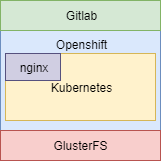
\includegraphics[width=0.3\textwidth]{figs/Infraestructura.png}
%	\caption{Infraestructura software propuesta.}\label{Infraestructura software propuesta}
%\end{figure}

\begin{landscape}
	\begin{figure}[H]
		\centering
		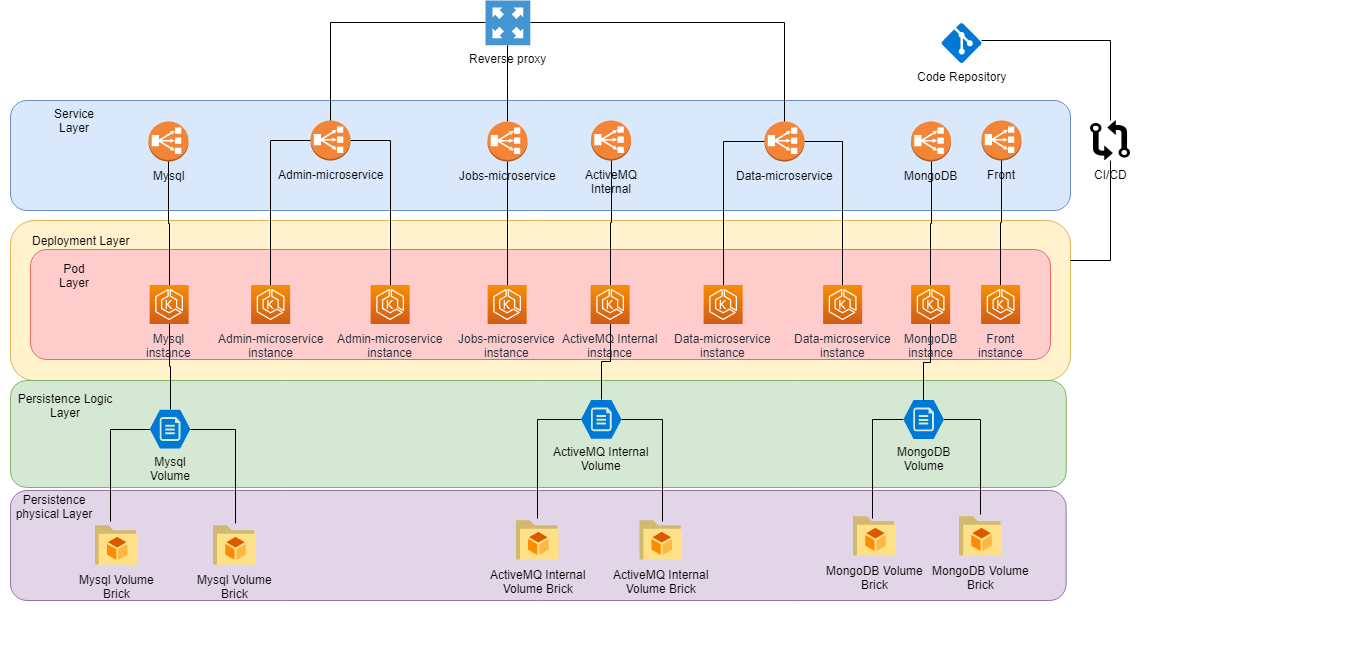
\includegraphics[width=1.5\textwidth]{figs/Thesis-Architecture.png}
		\caption{Arquitectura propuesta.}\label{Arquitectura propuesta}
	\end{figure}
\end{landscape}

\section{Prototipado}

\subsection{Configuraci\'on b\'asica cluster}
El cluster se conform� por 3 m�quinas f�sicas, sin embargo para la configuraci�n m�nima de alta disponibilidad se necesitaron 5 servidores, por lo cual la m�quina con m�s recursos se us� para la virtualizaci�n de 3 m�quinas con KVM\citep{kvmVirtualization} como podemos ver en la tabla \ref{tabla: Caracter�sticas de m�quinas en cluster} y en la figura \ref{Infraestructura hardware del prototipo}.


\begin{table}[H]
	\begin{minipage}{1\textwidth}
		\caption[Caracter�sticas de m�quinas en cluster]{ \raggedright Caracter�sticas de m�quinas en cluster}
		\label{tabla: Caracter�sticas de m�quinas en cluster}
		\begin{center}
			\begin{tabular}{ p{4cm}   p{5cm}  p{2cm}  p{3cm}  }
				\hline
				Nombre de dominio & CPU & \# Cores & RAM (GB) \\ \hline
				dns.local.cluster & Intel core i7 4720H & 1 & 1 \\ 
				glusterfs.local.cluster & Intel core i7 4720H & 1 & 0.59 \\ 
				master1.local.cluster & Intel core i7 4720H & 4 & 5.781 \\ 
				node1.local.cluster & Intel core i5 3230M & 4 & 5.697 \\ 
				node2.local.cluster & Intel core i3 4005U & 4 & 3.223 \\ \hline
			\end{tabular}
		\end{center}
	\end{minipage}
\end{table}
Para cada uno de las m�quinas se configur� la ip de forma est�tica y una clave RSA, la cual ser� usada posteriormente para el acceso remoto a los mismos.

\begin{figure}[H]
	\centering
	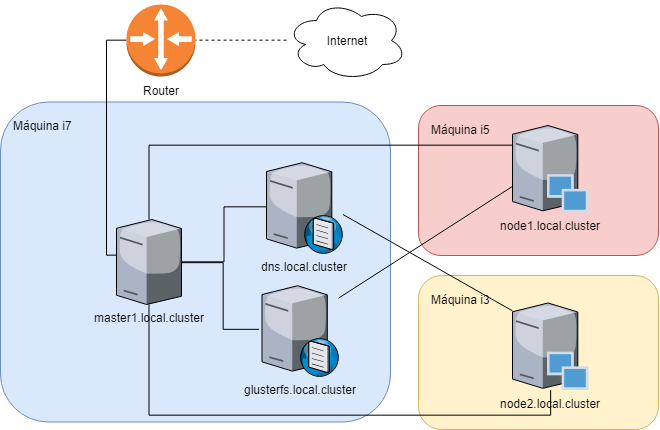
\includegraphics[width=\textwidth]{figs/arquitectura_infraestructura.png}
	\caption{Infraestructura hardware del prototipo.}
	\label{Infraestructura hardware del prototipo}
\end{figure}
\subsection{Configuraci\'on infraestructura cluster}
\subsubsection{Servidor DNS}
Se utiliz� la m�quina dns.local.cluster como servidor DNS usando bind\citep{dnsConfiguration} con la siguiente configuraci�n:



\begin{table}[H]
	\begin{minipage}{1\textwidth}
		\caption[Resoluci�n de nombres en cluster]{ \raggedright Resoluci�n de nombres en cluster}
		\label{tabla: Resoluci�n de nombres en cluster}
		\begin{center}
			\begin{tabular}{ p{5cm}   p{5cm}  }
				\hline
				Nombre de dominio & IP \\ \hline
				dns.local.cluster & 192.168.0.133 \\ 
				glusterfs.local.cluster & 192.168.0.134 \\ 
				master1.local.cluster & 192.168.0.130 \\ 
				node1.local.cluster & 192.168.0.131 \\ 
				node2.local.cluster & 192.168.0.132 \\ \hline
			\end{tabular}
		\end{center}
	\end{minipage}
\end{table}
Adicionalmente se instal� glusterfs para posteriormente distribuir el almacenamiento entre los servidores glusterfs.local.cluster y dns.local.cluster.
\subsubsection{Servidor Glusterfs}
Junto con el equipo de desarrollo de la plataforma IoT se definieron los siguientes artefactos a desplegar dentro de la infraestructura.
\begin{itemize}
	\item Proxy Reverso
	\item Servidor Mysql
	\item Servidor MongoDB
	\item Servidor ActiveMQ
	\item Microservicios
	\item Front
\end{itemize}





Posteriormente se clasificaron los artefactos seg�n la necesidad de persistir informaci�n de la siguiente forma:
\begin{table}[H]
	\begin{minipage}{1\textwidth}
		\caption[Artefactos de la aplicaci�n IoT seg�n su persistencia]{ \raggedright Artefactos de la aplicaci�n IoT seg�n su persistencia}
		\label{tabla: Artefactos de la aplicaci�n IoT seg�n su persistencia}
		\begin{center}
			\begin{tabular}{ p{7cm}   p{7cm}  }
				\hline
				Con persistencia & Sin persistencia  \\ \hline
				Servidor Mysql & Proxy Reverso \\
				Servidor MongoDB & Front  \\ 
				Servidor ActiveMQ & Microservicios  \\ \hline
			\end{tabular}
		\end{center}
	\end{minipage}
\end{table}

En nuestra arquitectura se escogi� GlusterFS como el sistema de archivos distribuidos, por lo que para cada uno de los artefactos de la arquitectura que requieren persistencia, se configur� un volumen GlusterFS de la siguiente forma:

\begin{table}[H]
	\begin{minipage}{1\textwidth}
		\caption[Configuraci�n de bricks de vol�menes]{ \raggedright Configuraci�n de bricks GlusterFS}
		\label{tabla: Configuraci�n de bricks GlusterFS}
		\begin{center}
			\begin{tabular}{ p{5cm}   p{3cm}  p{3cm} p{3cm}  }
				\hline
				Volumen & Usuario Id & Grupo Id & Permisos \\ \hline
				activemq & 0 & 0 & 755\\
				mongo & 184 & 184 & 777 \\ 
				mysql & 27 & 0 & 777 \\ \hline
			\end{tabular}
		\end{center}
	\end{minipage}
\end{table}

Finalmente se crea cada uno de los vol�menes con bricks tanto en el servidor dns.local.cluster como en glusterfs.local.cluster de tal forma que si alguno de los 2 servidores falla, est� el otro servidor para proveer los archivos y as� asegurar en ese caso la disponibilidad del sistema.



\subsubsection{Nodos}
Openshift Origin provee 2 m�todos de instalaci�n: Basado en paquetes RPM y basado en un sistema de contendores\citep{openshiftdocsInstallation}. 

Sin embargo la instalaci�n por sistema de contenedores requiere de acceso al repositorio privado de contenedores de Red Hat, por lo que se decidi� usar la instalaci�n basada en paquetes RPM.

La instalaci�n se realiz� usando Ansible con el archivo Inventory del anexo \ref{appendix:Archivo Inventory}. En este archivo definimos las diferentes m�quinas y su rol dentro de la infraestructura. 

Posteriormente se ejecutaron los siguientes ansible-playbook:
\begin{enumerate}
	\item {\textbf{prerequisites.yaml}} Instala y actualiza los paquetes software necesarios para la instalaci�n del cluster.
	\item {\textbf{deploy\_cluster.yaml}} Instala e inicia el cluster dentro de la infraestructura.
\end{enumerate}

Luego se modific� el archivo /etc/origin/master/htpasswd, a�adiendo el usuario 'admin' con contrase�a 'admin'.

Finalmente se ingresa a la plataforma web de administraci�n de Openshift como se ve en la imagen \ref{Plataforma web de administraci�n de Openshift}.


\begin{figure}[H]
	\centering
	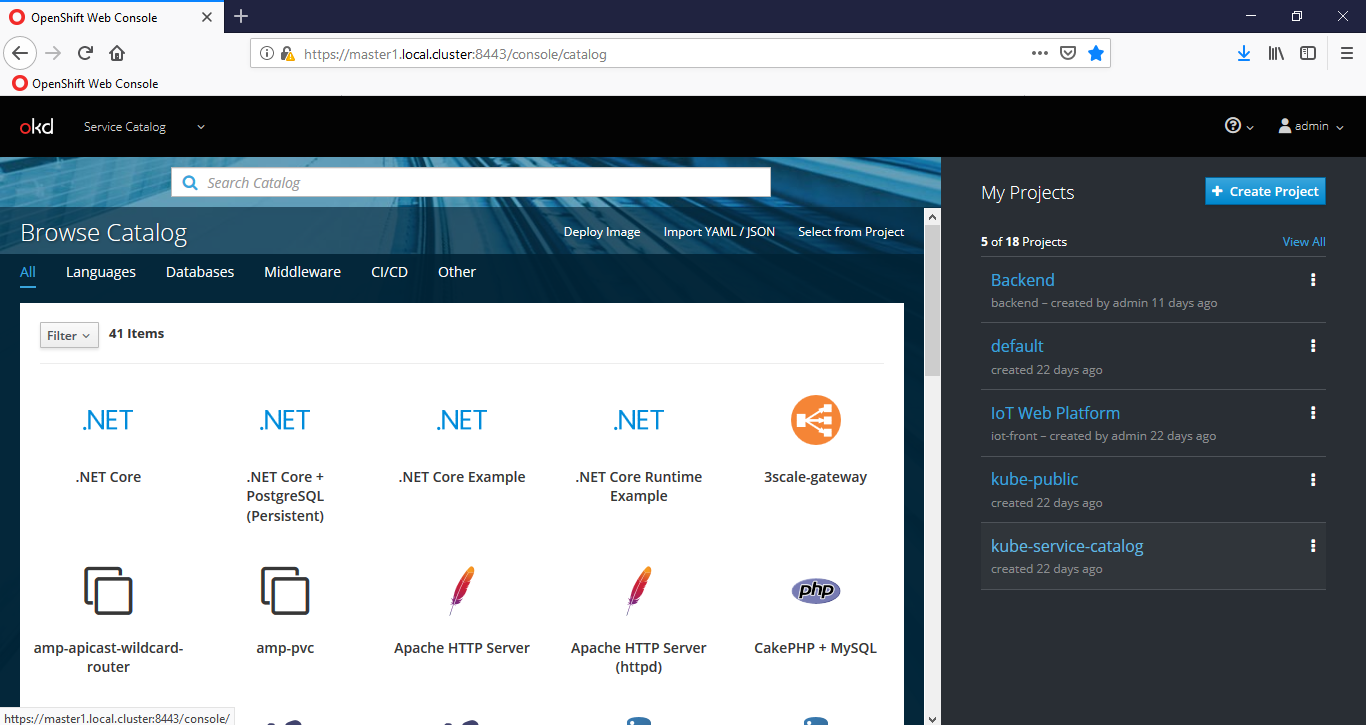
\includegraphics[width=\textwidth]{figs/openshift_console.PNG}
	\caption{Plataforma web de administraci�n de Openshift.}
	\label{Plataforma web de administraci�n de Openshift}
\end{figure}


Seguidamente, se crearon 2 proyectos: iot-front y backend. \\

\begin{lstlisting}[language=bash]
[root@master1 ~]# oc new-project iot-front
Now using project "iot-front" on server "https://master1.local.cluster:8443".
[root@master1 ~]# oc new-project backend
Now using project "backend" on server "https://master1.local.cluster:8443".
\end{lstlisting}



Finalmente, se despleg� el archivo gluster-endpoints.yaml del anexo \ref{appendix:Archivos de despliegue: Endpoints glusterfs} en el proyecto backend para registrar los nodos en los cuales se encuentran configurados los bricks de GlusterFS. \\
\begin{lstlisting}[language=bash]
[root@master1 ~]# oc project backend
Now using project "backend" on server "https://master1.local.cluster:8443".
[root@master1 ~]# oc create -f gluster-endpoints.yaml
endpoints/glusterfs-cluster created
\end{lstlisting}


\subsection{Despliegue aplicaci\'on}

Durante el proyecto se defini� el siguiente proceso para el despliegue de un artefacto dentro de la arquitectura propuesta con el fin de simplificar el proceso de despliegue y facilitar la integraci�n de nuevos componentes a la arquitectura.

Los archivos de configuraci�n\footnote{Dockerfile, pv.yaml, pvc.yaml, deployment.yaml, service.yaml} para cada uno de los artefactos se encuentran en el anexo \ref{appendix:Archivos de despliegue}.

Adicionalmente se realiz� un manual de instalaci�n de la arquitectura disponible en el anexo \ref{appendix:Manual de instalacion}.

\begin{landscape}
	\begin{figure}[H]
		\centering
		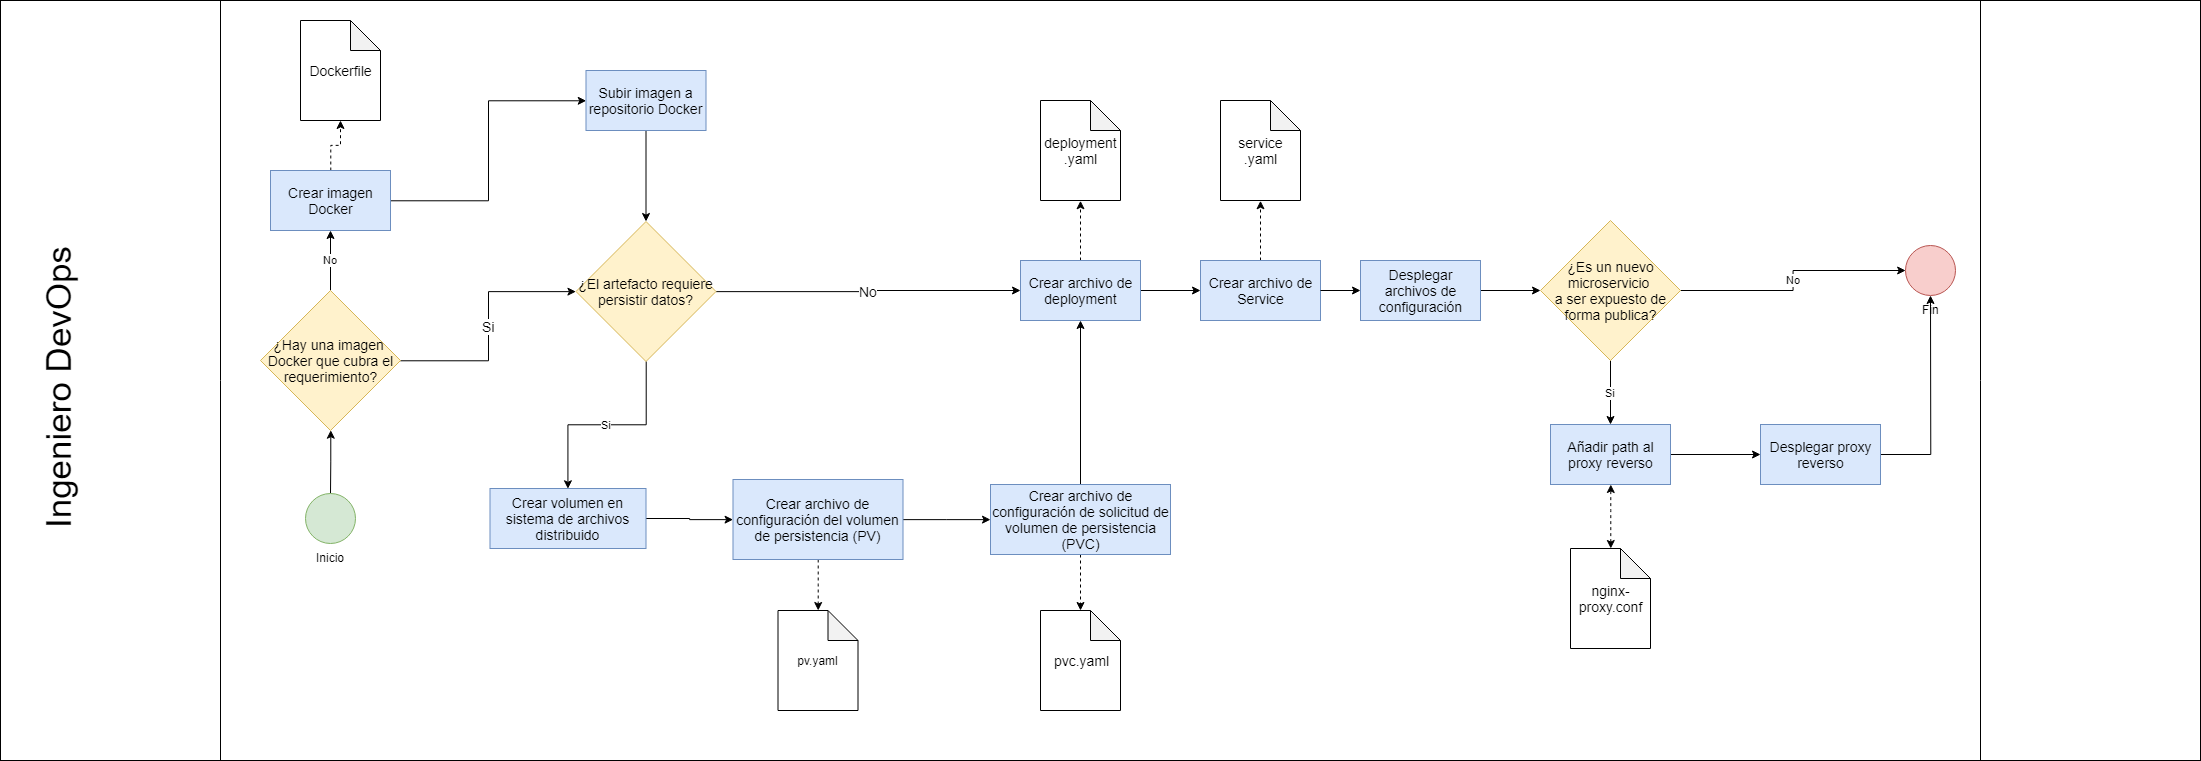
\includegraphics[width=1.3\textwidth]{figs/Proceso-de-despliegue-de-un-artefacto-2.png}
		\caption{Proceso de despliegue de un artefacto dentro de la arquitectura propuesta en BPMN.}
		\label{Proceso de despliegue de un artefacto dentro de la arquitectura propuesta en BPMN}
	\end{figure}
\end{landscape}

\subsection{Automatizaci\'on del proceso de despliegue}
Para realizar la automatizaci�n del proceso de despliegue se realiz� usando GitLab CI/CD. En el proyecto se tienen 2 automatizaciones de despliegue, una para el proyecto del front y otro para el proyecto del back. Estos se encuentran en el anexo \ref{appendix:Archivos de configuracion de despliegue continuo}.

Se definieron 3 etapas:
\begin{enumerate}
	\item {\textbf{Build:}} En esta etapa se compila y ejecutan los casos de prueba del c�digo a desplegar.
	\item {\textbf{Publish:}} En esta etapa se crea de forma autom�tica los contenedores con el c�digo compilado y se publican en Docker Hub.
	\item{\textbf{Deploy:}} En esta etapa se actualiza y despliega el archivo de deployment.yaml en el cluster.
\end{enumerate}

De esta manera, cada vez que los desarrolladores realizan un cambio sobre la rama 'master', autom�ticamente se ejecutan las 3 etapas para el despliegue de la aplicaci�n en el cluster. En caso de haber un error, Gitlab env�a un correo a los miembros del proyecto indicando que hubo un problema durante el despliegue.


\begin{figure}[H]
	\centering
	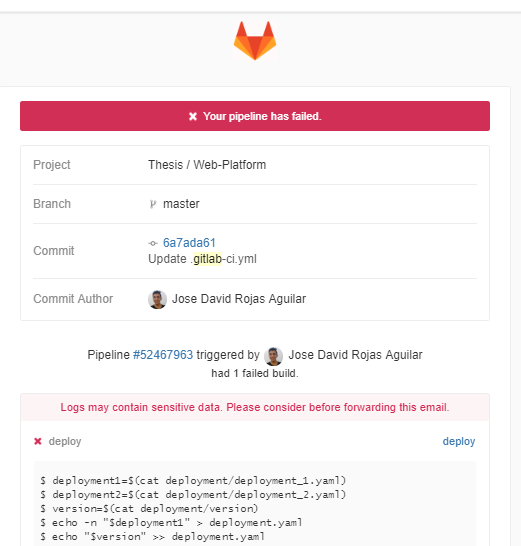
\includegraphics[width=0.35\textwidth]{figs/gitlab-error.png}
	\caption{Mensaje enviado por Gitlab cuando ocurre un error durante el despliegue autom�tico.}
	\label{Mensaje enviado por Gitlab cuando ocurre un error durante el despliegue autom�tico}
\end{figure}

\subsection{Implementaci\'on de pruebas}
Para la implementaci�n de las pruebas se realiz� el siguiente plan de pruebas con Jmeter. El plan de pruebas consisti� en enviar una solicitud para crear, consultar, modificar y eliminar un usuario. 

\begin{figure}[H]
	\centering
	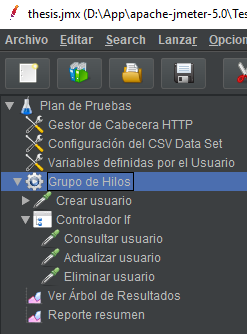
\includegraphics[width=0.35\textwidth]{figs/Jmeter-test.png}
	\caption{Plan de pruebas implementado en Jmeter.}
	\label{Plan de pruebas implementado en Jmeter}
\end{figure}

La actividad 'Reporte resumen' fue la fuente de los datos presentados en los resultados de la ejecuci�n de las pruebas.

\section{Validaci\'on de prototipo}
\subsection{Aplicaci\'on pruebas}
Los resultados de las pruebas se consignaron en las tablas \ref{tabla: Porcentaje de solicitudes fallidas durante un despliegue}, \ref{tabla: Tiempo promedio de respuesta para 1000 solicitudes por minuto}, \ref{tabla: N�mero m�ximo de solicitudes por minuto sin solicitudes fallidas.}, \ref{tabla: Porcentaje de solicitudes fallidas para 3500 solicitudes por minuto} y \ref{tabla: Cantidad de solicitudes fallidas para 1000 solicitudes por minuto durante el fallo de un nodo}.

\begin{table}[H]
	\begin{minipage}{1\textwidth}
		\caption[Porcentaje de solicitudes fallidas durante un despliegue]{ \raggedright Porcentaje de solicitudes fallidas durante un despliegue}
		\label{tabla: Porcentaje de solicitudes fallidas durante un despliegue}
		\begin{center}
			\begin{tabular}{ p{7cm}   p{7cm}  }
				\hline
				Escenario &  \%  \\ \hline
				Monol�tico & 4.45  \\ 
				1 instancia & 10.51  \\ 
				2 instancias & 2.26  \\ 
				3 instancias & 2.30 \\ \hline
			\end{tabular}
		\end{center}
	\end{minipage}
\end{table}
\begin{table}[H]
	\begin{minipage}{1\textwidth}
		\caption[Tiempo promedio de respuesta para 1000 solicitudes por minuto]{ \raggedright Tiempo promedio de respuesta para 1000 solicitudes por minuto}
		\label{tabla: Tiempo promedio de respuesta para 1000 solicitudes por minuto}
		\begin{center}
			\begin{tabular}{ p{7cm}   p{7cm}  }
				\hline
				Escenario &  Milisegundos  \\ \hline
				Monol�tico & 413 \\ 
				1 instancia & 455  \\ 
				2 instancias & 434  \\ 
				3 instancias & 419 \\ \hline
			\end{tabular}
		\end{center}
	\end{minipage}
\end{table}
\begin{table}[H]
	\begin{minipage}{1\textwidth}
		\caption[N�mero m�ximo de solicitudes por minuto sin solicitudes fallidas.]{ \raggedright N�mero m�ximo de solicitudes por minuto sin solicitudes fallidas.}
		\label{tabla: N�mero m�ximo de solicitudes por minuto sin solicitudes fallidas.}
		\begin{center}
			\begin{tabular}{ p{7cm}   p{7cm}  }
				\hline
				Escenario &  Solicitudes por minuto  \\ \hline
				Monol�tico & 2690 \\ 
				1 instancia & 2616  \\ 
				2 instancias & 3800  \\ 
				3 instancias & 4320 \\ \hline
			\end{tabular}
		\end{center}
	\end{minipage}
\end{table}
\begin{table}[H]
	\begin{minipage}{1\textwidth}
		\caption[Porcentaje de solicitudes fallidas para 3500 solicitudes por minuto]{ \raggedright Porcentaje de solicitudes fallidas para 3500 solicitudes por minuto}
		\label{tabla: Porcentaje de solicitudes fallidas para 3500 solicitudes por minuto}
		\begin{center}
			\begin{tabular}{ p{7cm}   p{7cm}  }
				\hline
				Escenario &  \%  \\ \hline
				Monol�tico & 24.26 \\ 
				1 instancia & 36.28  \\ 
				2 instancias & 0  \\ 
				3 instancias & 0 \\ \hline
			\end{tabular}
		\end{center}
	\end{minipage}
\end{table}
\begin{table}[H]
	\begin{minipage}{1\textwidth}
		\caption[Cantidad de solicitudes fallidas para 1000 solicitudes por minuto durante el fallo de un nodo]{ \raggedright Cantidad de solicitudes fallidas para 1000 solicitudes por minuto durante el fallo de un nodo}
		\label{tabla: Cantidad de solicitudes fallidas para 1000 solicitudes por minuto durante el fallo de un nodo}
		\begin{center}
			\begin{tabular}{ p{7cm}   p{7cm}  }
				\hline
				Escenario &  Solicitudes fallidas  \\ \hline
				Monol�tico & 172,9 \\ 
				1 instancia & 157,2  \\ 
				2 instancias & 77  \\ 
				3 instancias & 60 \\ \hline
			\end{tabular}
		\end{center}
	\end{minipage}
\end{table}
\subsection{An\'alisis resultados}
\begin{itemize}
	\item Durante la prueba de la tabla \ref{tabla: Porcentaje de solicitudes fallidas durante un despliegue}, la mayor cantidad de solicitudes fallidas se evidenci� en el ambiente de 1 instancia ya que este no es compatible con el despliegue en release de Kubernetes. Los ambientes de 2 y 3 instancias soportaban el tr�fico entrante con la versi�n anterior mientras la nueva versi�n estaba lista.
	\item El ambiente monol�tico tiene el tiempo de respuesta m�s �ptimo en la prueba de la tabla \ref{tabla: Tiempo promedio de respuesta para 1000 solicitudes por minuto} ya que este ambiente no debe realizar transferencia de datos por medio de la red.
	\item El n�mero m�ximo de solicitudes es proporcional a la cantidad de instancias ya que el tr�fico se distribuye en las mismas.
	\item Durante la prueba de la tabla \ref{tabla: Porcentaje de solicitudes fallidas para 3500 solicitudes por minuto} se evidenci� que un ambiente monol�tico tiene un mayor rendimiento que un ambiente 1 instancia ya que el ambiente monol�tico debe transferir datos por medio de la red, lo cual impacta significativamente en su rendimiento. 
	\item Como vemos en la tabla \ref{tabla: Cantidad de solicitudes fallidas para 1000 solicitudes por minuto durante el fallo de un nodo}, la redundancia de recursos es fundamental para disminuir el impacto de un fallo en la respuesta de las solicitudes.
	\item A partir de 2 instancias, la carga se distribuye entre los diferentes servidores, lo cual lleva a una mejora significativa en el rendimiento de la arquitectura.
	\item La mejora de rendimiento entre 1 instancia y 2 instancias es mucho m�s significativa que la mejora entre 2 instancias y 3 instancias. Esto se debe a que para el primer caso, hay un cambio en la distribuci�n de carga entre los servidores f�sicos, mientras que en el segundo caso, no hay un cambio de carga a nivel f�sico ya que siguen siendo 2 servidores f�sicos, el cambio se da a nivel software.
\end{itemize}
   	% Desarrollo del proyecto
% ------------------------------------------------------------------------
% ------------------------------------------------------------------------
% ------------------------------------------------------------------------
%                            Trabajo futuro
% ------------------------------------------------------------------------
% ------------------------------------------------------------------------
% ------------------------------------------------------------------------

\chapter{Trabajo futuro}
% ------------------------------------------------------------------------
\noindent Actividades complementarias a los desarrollos presentados, incluyen el c�lculo autom�tico para conjuntos estabilizantes en plantas arbitrarias empleando el \emph{m�todo de la signatura} desarrollado por Keel y Bhattacharyya en \citep{keel2008}.\\

Asimismo es importante explorar otras topologias de compensador y controladores PID, en sus versiones de tiempo continuo y discreto.
% ------------------------------------------------------------------------    	% Conclusiones
% ------------------------------------------------------------------------
% ------------------------------------------------------------------------
% ------------------------------------------------------------------------
%                             Conclusiones
% ------------------------------------------------------------------------
% ------------------------------------------------------------------------
% ------------------------------------------------------------------------

\chapter{Conclusiones}
% ------------------------------------------------------------------------
% ------------------------------------------------------------------------
\noindent A partir de los desarrollos presentados y los resultados obtenidos en el presente trabajo de grado, es posible enunciar las siguientes conclusiones:
% ------------------------------------------------------------------------
\begin{itemize}
  \item[ ] Se interpretaron las tablas de dise�o de par�metros PI de \emph{Ziegler \& Nichols} en t�rminos de conjuntos estabilizantes. Tal y como fue abordado en la \emph{Secci�n} \ref{estabanalpi}, se ilustr� el dise�o de un compensador PI para una planta y posteriormente se analiz� la posici�n de dicho punto en el plano $\left(k_P, k_I \right)$ de controladores factibles con base en su conjunto estabilizante. A partir de ello, es claro que el m�todo de \emph{Ziegler \& Nichols} siempre dar� como resultado un controlador estable, tomando en cuenta su caracter emp�rico. Sin embargo, a partir de la definici�n de una m�trica en la \emph{Secci�n} \ref{metrdef}, fue posible mostrar a trav�s de una cuantificaci�n para su \emph{fragilidad} que no necesariamente el controlador calculado es estable ante ligeras variaciones en sus valores de par�metro. De otro lado, la definici�n de conjunto estabilizante fue ampliamente abordada en la \emph{Secci�n} \ref{conjestabsect} y posteriormente aplicada al caso PI en la \emph{Secci�n} \ref{estabanalpi}.
  \item[ ] Se desarroll� un algoritmo que permiti� verificar las condiciones de estabilidad para controladores PI dise�ados mediante el m�todo de \emph{Ziegler \& Nichols}. Inicialmente, se realiz� una discusi�n general de conjuntos estabilizantes en la \emph{Secci�n} \ref{conjestabsect}, posteriormente complementada en la \emph{Secci�n} \ref{conjestabpi} con medidas de inestabilidad a trav�s de una m�trica basada en la interpretaci�n geom�trica para m�rgenes de estabilidad en un lazo de control sometido a control PI. El m�todo (o algoritmo) consisti� fundamentalmente en calcular el conjunto estabilizante en el plano de par�metros del controlador, para posteriormente transformar las especificaciones de controladores viables a cantidades igualmente viables en el dominio del tiempo. Posteriormente un usario podr�a seleccionar el controlador deseado a partir de un punto en el conjunto de par�metros admisible, para el cual se provee adem�s indicaci�n de sus m�rgenes de estabilidad como medida de \emph{fragilidad}. El procedimiento anterior se desarroll� para los casos de un compensador de 3 par�metros (uno de ellos conocido) y un controlador PI.
  \item[ ] Se implement� una interfaz para c�lculo de controladores PI a partir de selecci�n de par�metros en el dominio del tiempo, admisibles respecto al conjunto estabilizante correspondiente. El algoritmo descrito en el �tem anterior fue codificado en una interfaz en MATLAB seg�n se describe en la \emph{Secci�n} \ref{interfazsect}, empleando una metodolog�a de dise�o del tipo \emph{top-down}.
\end{itemize}
% ------------------------------------------------------------------------    	% Recomendaciones
\input{Secs/T8}   	% Limitaciones
% ------------------------------------------------------------------------
% Bibliograf�a
% ------------------------------------------------------------------------
\addcontentsline{toc}{chapter}{Referencias Bibliogr�ficas}\newpage
\bibliographystyle{apalike}
\bibliography{xbib}
% ------------------------------------------------------------------------
% Anexos
% ------------------------------------------------------------------------

\newpage
\nnchapter{Ap�ndices}
% ------------------------------------------------------------------------
\anexo{Fundamentos de s�lidos r�gidos}\label{anexoA}
% ------------------------------------------------------------------------
\noindent Un s�lido r�gido, es un cuerpo formado por varias part�culas puntuales que
guardan distancias constantes entre s� \citep{sears2005fisica}.\\

Una operaci�n fundamental para definir cantidades en el espacio de movimiento de
un s�lido r�gido es el producto vectorial (tambi�n denominado producto cruz \citep{stanley1993algebra}),
el cual produce un vector perpendicular (normal) al plano formado por otros dos vectores
que se multiplican.\\

Sean dos vectores $\vec{a}$ y $\vec{b}$ definidos en $\mathbb{R}^3$. El producto vectorial entre $\vec{a}$ y $\vec{b}$ (denotado $\vec{a} \times \vec{b}$) es otro vector (digamos $\vec{c} \in \mathbb{R}^3$) cuyo c�lculo puede ser efectuado a trav�s de determinantes como sigue:
% ------------------------------------------------------------------------
\begin{equation}\label{defprodvect}
\vec{c} = \vec{a} \times \vec{b} = \begin{vmatrix}
i& j & k \\
a_i & a_j  & a_k \\
b_i & b_j  & b_k
\end{vmatrix} =
\begin{vmatrix}
 a_j & a_k \\
 b_j & b_k
\end{vmatrix}i~
-
\begin{vmatrix}
a_i & a_k \\
b_i & b_k
\end{vmatrix}j~
+\begin{vmatrix}
 a_i & a_j \\
 b_i & b_j
\end{vmatrix}k
\end{equation}
% ------------------------------------------------------------------------
De esta manera, siendo $\vec{a}=(1,-1,2)$ y $\vec{b}=(3,-4,5)$ se obtiene:
% ------------------------------------------------------------------------
\begin{equation}
\vec{a} \times \vec{b} =\begin{vmatrix}
i& j & k \\
1 &-1  &2 \\
3 &-4  &5
\end{vmatrix}=
\begin{vmatrix}
 -1&2 \\
 -4&5
\end{vmatrix}i~
-
\begin{vmatrix}
1 &2 \\
3 &5
\end{vmatrix}j~
+\begin{vmatrix}
 1&-1 \\
 3&4
\end{vmatrix}k
= 3i-j-k
\end{equation}
% ------------------------------------------------------------------------
La Fig. \ref{prodvect} ilustra esta operaci�n gr�ficamente en el espacio tridimensional.
% ------------------------------------------------------------------------
\begin{figure}[h]
\centering
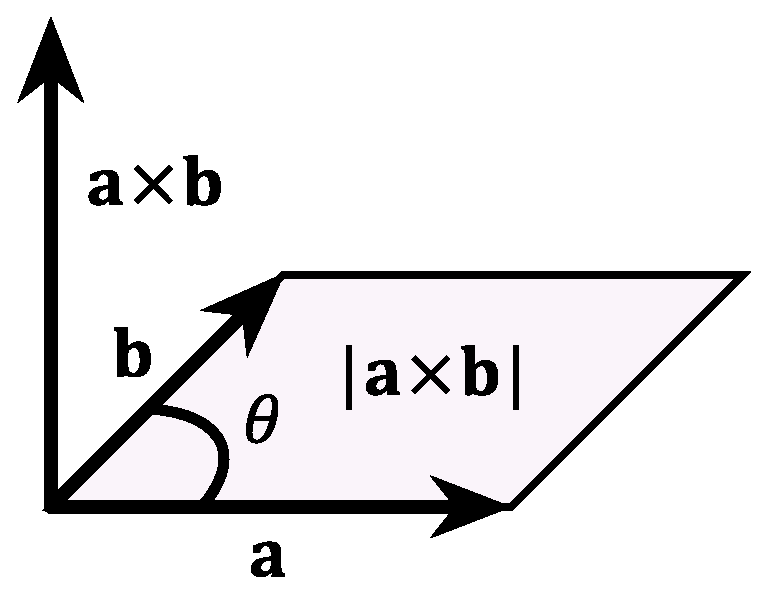
\includegraphics[width=0.3\textwidth]{Figs/prodvect}
\caption[]{Ilustraci�n gr�fica para producto vectorial}\label{prodvect}
\end{figure}
% ------------------------------------------------------------------------

\section*{Condici�n de rigidez}
% ------------------------------------------------------------------------
\noindent Considere el s�lido r�gido presentado en la Fig. \ref{rigid}. Para cada pareja de puntos $(P_i, P_j)$ pertenecientes al s�lido, se cumple:
% ------------------------------------------------------------------------
\begin{equation}\label{rigidez}
\frac{d}{dt}[\left|r_i - r_j\right|] = \frac{d}{dt}[\left|r_{ij}\right|] = 0,
\end{equation}
% ------------------------------------------------------------------------
lo cual significa que la distancia entre puntos de un s�lido r�gido se mantiene invariante. Esto �ltimo se conoce como la \emph{condici�n de r�gidez}.\\
% ------------------------------------------------------------------------
\begin{figure}[h]
\centering
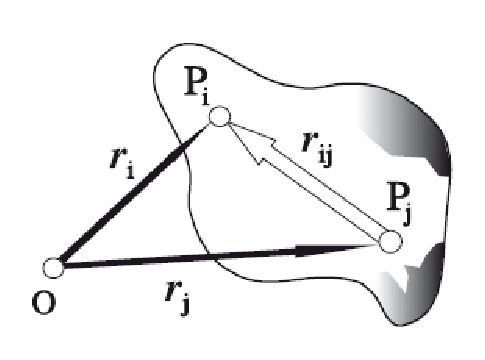
\includegraphics[width=0.3\textwidth]{Figs/rigid}
\caption[]{S�lido r�gido}\label{rigid}
\end{figure}
% ------------------------------------------------------------------------

Asimismo, a partir de \eqref{rigidez} se obtiene:
% ------------------------------------------------------------------------
\begin{equation}
\frac{d}{dt}[\left|r_i - r_j\right|] = \left|\dot{r}_i - \dot{r}_j\right| = 0,
\end{equation}
% ------------------------------------------------------------------------
y por tanto, sabiendo que $\vec{\dot{r}}$ es el vector velocidad $\vec{v}$ para un punto del s�lido visto desde el observador, es posible escribir:
% ------------------------------------------------------------------------
\begin{equation}
\left|v_i\right| = \left|v_j\right|,
\end{equation}
% ------------------------------------------------------------------------
con lo cual la velocidad de traslaci�n para cualquier punto del s�lido ser� la misma, y as�, una vez definido el movimiento de un punto cualquiera del cuerpo rigido que se traslada en el espacio, es posible definir la totalidad de su movimiento.

% ------------------------------------------------------------------------
\section*{Movimiento de rotaci�n}
% ------------------------------------------------------------------------
\noindent En la Fig. \ref{rotacion} se ilustra un punto que rota alrededor de un eje fijo, localizado en el cuerpo del s�lido.\\
% ------------------------------------------------------------------------
\begin{figure}[h]
\centering
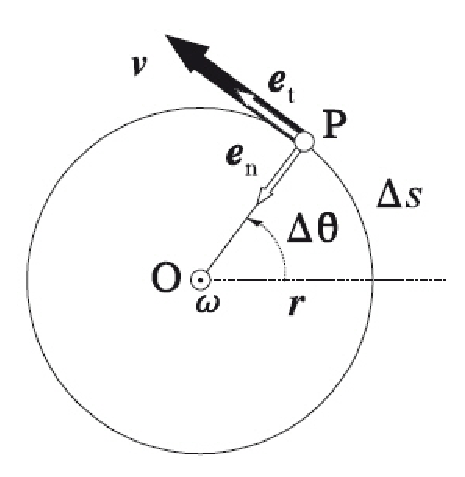
\includegraphics[width=0.3\textwidth]{Figs/rotacion}
\caption[]{Rotaci�n de un punto del s�lido alrededor de un eje fijo}\label{rotacion}
\end{figure}
% ------------------------------------------------------------------------

A partir de ello, es posible definir la velocidad angular que experimenta el punto $P$ alrededor del eje de rotaci�n, en el modo siguiente:
% ------------------------------------------------------------------------
\begin{equation}
\omega = \frac{d}{dt}\theta
\end{equation}\
% ------------------------------------------------------------------------

Tambien, puede escribirse del diagrama la velocidad tangencial $v$ del punto mediante:
% ------------------------------------------------------------------------
\begin{equation}
\vec{v} = \vec{r} \times \vec{\omega},
\end{equation}
% ------------------------------------------------------------------------
siendo $\vec{r}$ el vector que marca la distancia del punto $P$ al eje de rotaci�n $O$.\\

Por tanto, el vector de aceleraci�n puede ser formulado como:
% ------------------------------------------------------------------------
\begin{eqnarray}\label{aceler}
\nonumber \frac{d}{dt}\vec{v} & = & \frac{d}{dt}[\vec{r} \times \vec{\omega}]\\
\nonumber & = & \left( \frac{d}{dt}\vec{r}\times \vec{\omega}\right) + \left( \vec{r}\times \frac{d}{dt}\vec{\omega}\right)\\
\vec{a}   & = & \vec{r} \times \vec{\alpha},
\end{eqnarray}
% ------------------------------------------------------------------------
con $\vec{a}$ y $\vec{\alpha}$ representando, respectivamente, los vectores de aceleraci�n lineal y angular. Note que se asume $\frac{d}{dt}\vec{r} = 0$ debido a que el eje de rotaci�n es fijo.

% ------------------------------------------------------------------------
\section*{Conservaci�n del momento angular}
% ------------------------------------------------------------------------
\noindent En un movimiento traslacional, el principio de conservaci�n del momento lineal establece:
% ------------------------------------------------------------------------
\begin{equation}
\frac{d}{dt}\vec{p} = \frac{d}{dt}{m\vec{v}} = 0,
\end{equation}
% ------------------------------------------------------------------------
a partir de lo cual el momento $\vec{p}$ ser� constante en ausencia de fuerzas externas.\\

De manera similar, es posible definir el momento angular $\vec{\mathbf{L}}$ de una part�cula de masa puntual que rota alrededor de un eje fijo, en el modo siguiente:
% ------------------------------------------------------------------------
\begin{equation}\label{momang}
\vec{\mathbf{L}} = \vec{r} \times \vec{p},
\end{equation}
% ------------------------------------------------------------------------
siendo $\vec{r}$ el vector de distancia a la masa desde el centro de rotaci�n.\\

Por tanto, el principio de conservaci�n del momento angular puede establecerse como sigue:
% ------------------------------------------------------------------------
\begin{eqnarray*}
\frac{d}{dt}\vec{\mathbf{L}} & = & \frac{d}{dt}{[\vec{r} \times \vec{p}]} \\
                             & = & \frac{d}{dt}{[\vec{r} \times m\vec{v}]}\\
                             & = & m \frac{d}{dt}{[\vec{r} \times \vec{v}]}\\
                             & = & m\left([\vec{r}\times\frac{d}{dt}\vec{v}]+[\frac{d}{dt}\vec{r}\times\vec{v}]\right)\\
                             & = & m\left([\vec{r}\times \vec{a}]+[\vec{v}\times\vec{v}]\right)\\
                             & = & \vec{r}\times m\vec{a}\\
                             & = & \vec{r}\times \vec{F}\\
                             & = & \tau,
\end{eqnarray*}
% ------------------------------------------------------------------------
siendo $\tau$ el torque neto aplicado.\\

Empleando \eqref{aceler} puede relacionarse este torque con la aceleraci�n angular $\vec{\alpha}$, a partir de:
% ------------------------------------------------------------------------
\begin{eqnarray*}
\tau & = & \vec{r}\times m\vec{a}\\
     & = & \vec{r}\times m\left(\vec{r} \times \vec{\alpha}\right)\\
     & = & m\left(\vec{r}\times \left(\vec{r} \times \vec{\alpha}\right)\right)
\end{eqnarray*}
% ------------------------------------------------------------------------
donde, si $\vec{r}$ es perpendicular a $\vec{\alpha}$, entonces el producto vectorial se reduce al producto de las magnitudes:
% ------------------------------------------------------------------------
\begin{eqnarray}\label{newrot}
\nonumber \tau & = & m r^2 \alpha \\
               & = & I \alpha,
\end{eqnarray}
% ------------------------------------------------------------------------
siendo $I$ el momento de inercia de las partes rotativas del cuerpo r�gido.\\

La expresi�n \eqref{newrot} es la segunda ley de Newton de rotaci�n, y podr� ser definida siempre que sea v�lido un $I$ constante. Dicha situaci�n no siempre es posible, principalmente si se asume que el eje de rotaci�n puede variar en el tiempo. En tal caso, $\vec{r}$ en la Fig. \ref{rotacion} no es constante y por tanto no es v�lida la soluci�n propuesta para $\vec{a}$ en \eqref{aceler}, resultando en la siguiente definici�n alternativa para $\tau$:
% ------------------------------------------------------------------------
\begin{eqnarray*}
\tau & = & \vec{r}\times m\vec{a}\\
     & = & \vec{r}\times m\left(\left( \frac{d}{dt}\vec{r}\times \vec{\omega}\right) + \left( \vec{r}\times \frac{d}{dt}\vec{\omega}\right)\right)\\
     & = & m\left(\left[\vec{r}\times\left( \frac{d}{dt}\vec{r}\times \vec{\omega}\right)\right] + \left[\vec{r}\times\left( \vec{r}\times \vec{\alpha}\right)\right]\right)\\
     & = & m\left(\left[\vec{r}\times\left( \frac{d}{dt}\vec{r}\times \vec{\omega}\right)\right]\right) + I\alpha.
\end{eqnarray*}\
% ------------------------------------------------------------------------

El t�rmino
% ------------------------------------------------------------------------
$$
m\left(\left[\vec{r}\times\left( \frac{d}{dt}\vec{r}\times \vec{\omega}\right)\right]\right),
$$\
% ------------------------------------------------------------------------
representa los efectos (torques) debidos a las variaciones del eje de rotaci�n, que evidentemente tambi�n representan variaciones del vector de momento angular $\vec{\mathbf{L}}$. Dichos efectos se denominan \emph{fuerzas inerciales}, puesto que tienen sentido en un marco de referencia de un cuerpo en rotaci�n. Los tipos m�s representativos de fuerza inercial son los efectos girosc�picos y la fuerza de Coriollis \citep{sears2005fisica}.
% ------------------------------------------------------------------------  % Fundamentos de s�lidos r�gidos

\newpage
\anexo{Archivo Inventory}\label{appendix:Archivo Inventory}
\begin{minted}[
	gobble=4,
	frame=single,
	linenos,
	breaklines
	]{yaml}
				[OSEv3:children]
				masters
				nodes
				etcd
				[OSEv3:vars]
				ansible_ssh_user=root
				openshift_deployment_type=origin
				openshift_master_identity_providers=[{'name': 'htpasswd_auth', 'login': 'true', 'challenge': 'true', 'kind': 'HTPasswdPasswordIdentityProvider'}]
				openshift_disable_check=memory_availability,disk_availability
				[masters]
				master1.local.cluster
				[etcd]
				master1.local.cluster
				[nodes]
				master1.local.cluster openshift_node_group_name='node-config-master-infra'
				node1.local.cluster openshift_node_group_name='node-config-compute'
				node2.local.cluster openshift_node_group_name='node-config-compute'
\end{minted} % Funci�n ode45 de MATLAB
% ------------------------------------------------------------------------
% ------------------------------------------------------------------------
% ------------------------------------------------------------------------
%                                Anexo C
% ------------------------------------------------------------------------
% ------------------------------------------------------------------------
% ------------------------------------------------------------------------
% ------------------------------------------------------------------------
\newpage
\anexo{Endpoints glusterfs}\label{appendix:Archivos de despliegue: Endpoints glusterfs}


    \begin{minted}[
gobble=4,
frame=single,
linenos,
breaklines
]{yaml}
				apiVersion: v1
				kind: Endpoints
				metadata:
				name: glusterfs-cluster
				subsets:
				- addresses:
				- ip: 192.168.0.133
				ports:
				- port: 1
				- addresses:
				- ip: 192.168.0.134
				ports:
				- port: 1
\end{minted}  
 % Interfaz de animaci�n de la din�mica del sistema
% ------------------------------------------------------------------------
\end{document}                                          % Fin de documento
% ------------------------------------------------------------------------ 